% This is samplepaper.tex, a sample chapter demonstrating the
% LLNCS macro package for Springer Computer Science proceedings;
% Version 2.20 of 2017/10/04
%
\documentclass[runningheads]{llncs}
%
\usepackage{multirow}
\usepackage{graphicx}
\usepackage{textcomp}
% Used for displaying a sample figure. If possible, figure files should
% be included in EPS format.
%
% If you use the hyperref package, please uncomment the following line
% to display URLs in blue roman font according to Springer's eBook style:
% \renewcommand\UrlFont{\color{blue}\rmfamily}

\begin{document}
%
\title{AERoS: Framework for the Assurance of Emergent Behaviour for use in Autonomous Robotic Swarms\thanks{Supported by organization x.}}
%
%\titlerunning{Abbreviated paper title}
% If the paper title is too long for the running head, you can set
% an abbreviated paper title here
%
\author{Dhaminda B. Abeywickrama\inst{\dag}\inst{1}\orcidID{0000-0002-4423-0284} \and
James Wilson\inst{\dag}\inst{1}\orcidID{0000-0002-0758-6732} \and
Third Author\inst{1}\orcidID{2222--3333-4444-5555} \and
4th Author\inst{1}\orcidID{2222--3333-4444-5555} \and
5th Author\inst{1}\orcidID{2222--3333-4444-5555} \and
6th Author\inst{1}\orcidID{2222--3333-4444-5555} \and
7th Author\inst{1}\orcidID{2222--3333-4444-5555} \and
8th Author\inst{1}\orcidID{2222--3333-4444-5555} \and
9th Author\inst{1}\orcidID{2222--3333-4444-5555}}
%
\authorrunning{F. Author et al.}
% First names are abbreviated in the running head.
% If there are more than two authors, 'et al.' is used.
%
\institute{University of Bristol, Bristol, UK}
%
\maketitle              % typeset the header of the contribution
%
\begin{abstract}

\keywords{First keyword  \and Second keyword \and Another keyword.}
\end{abstract}
%
%
%

\section{Introduction}\label{introduction}
The main contribution of this paper is a novel framework for assurance of emergent behaviour for use in autonomous robotic swarms based on the AMLAS, SOCA, and SACE* guidance (* under consideration). We illustrate our framework using a public cloakroom case study. 

%\\\noindent\textbf{\textit{[Author General Guidelines: please write as a paper not as a Guidance like AMLAS; Please do not use AERoS word]}}\\


\section{Background and Related Work}\label{background-relatedwork}


\subsection{Background}\label{background}




\subsubsection{Robotic Swarms}
%\noindent Autonomous
%\\ \noindent Large Number of agents (10+)
%\\ \noindent Relatively incapable individuals
%\\ \noindent Restrained Homogeneity
%\\ \noindent Minimal communication capabilities (Decentralised)

\subsubsection{Case Study: Cloakroom}\label{ex:cloakroom}

%\vspace{2mm}
%\noindent\textbf{\textit{\newline[Author Guidelines: Please use the cloakroom case study to illustrate the framework in Section III. If the examples in cloakroom case study are not sufficient, other swarm use cases listed below can be considered.]}}
% The case study describes a public cloakroom where swarm of robots assist customers looking to deposit their jackets at an event \cite{Jones2020}. 
% It describes cases where customers are depositing jackets, handing a jacket to a robot for storing, and retrieval of jackets back to the customer. 
A company that organizes bespoke events with 50 to 10000 attendees is looking to automate their cloakroom by deploying a swarm of robots to assist attendees (customers) to deposit, store and deliver their belongings (e.g. jackets) \cite{Jones2020}. % cloakroom paper 
%Mindful of the safety, operational and regulatory requirements of the healthcare sector
The system must prioritize public safety, and the company decides to use this standard on transparency as a draft specification for their engineers to more transparently communicate the decision-making processes of their automated cloakroom. %swarm system. 

% \paragraph*{Other Swarm Use Cases}
% \emph{\\Fault detection, diagnosis and recovery – Monitoring fires in a natural environment}. Fault detection model shall be trained to high level of accuracy. Thresholds for fault tolerance shall be set appropriately such that misclassification of a fault is a rare event. An agent experiencing minor faults shall not be immediately removed, should the fault not impact the task at hand. \\
% \emph{\noindent Social swarm – Brainstorming at an event}. Humans follow robots which cluster based on input. Minimise blocking paths of other humans and agents. Maintain situational awareness of humans and agents in the environment. Before the task, provide a clear explanation of the steps of the activity. Clear guidance during the task. Provide information about how the swarm/robot works.

% \noindent See research paper ``Mutual shaping in swarm robotics: User studies in fire and rescue, storage organisation, and bridge inspection" \cite{Carrillo-Zapata2020}.

\subsection{Related Work}\label{relatedwork}
%\subsubsection{Specification Challenges and Standards} 
%\subsection{Standards for Autonomous Systems}
%Dhaminda B. Abeywickrama: Needs to be trimmed and edited. 
Autonomous systems are systems that involve software applications, machines and people, which are capable of taking actions with no or little human supervision~\cite{Murukannaiah2020}. 
The functionality of an autonomous system (i.e. what it is meant to do, what it does, and what it could do) evolves or changes over time. 
One of the main issues of adopting current standards and regulations with autonomous systems is the lack of consideration to the notions of \textit{uncertainty} and \textit{autonomy} \cite{Fisher2021}. 
Most conventional processes for defining system requirements assume that these are fixed and can be defined in a complete and precise manner before the system goes into operation \cite{Abeywickrama2022}. 
Also, in existing standards and regulations, the notion of autonomy is not their most characterizing feature where they are neither driven nor strongly influenced by it \cite{Fisher2021}. 
Most existing standards are either implicitly or explicitly based on the V\&V model, which moves from requirements through design onto implementation and testing before deployment~\cite{Jia2021}. 
However, this model is unlikely to be suitable for systems with the ability to adapt their functionality in operation; e.g.\ through interaction with other agents and the environment (e.g. as is the case with swarms); or through experience-driven adaptation as is the case with machine learning \cite{Abeywickrama2022}. 
Autonomous systems with evolving functionality follow a different, much more iterative life-cycle. 
Thus, there is a need for new standards and assurance processes that extend beyond design time and allow continuous certification at runtime~\cite{Rushby2008}. 
In this context, lately, there have been several standards and guidance introduced by several industry committees and research groups. 
Now we provide an overview of several key efforts with any trustworthiness properties or ontologies supported by them.
%Now we provide an overview of several key efforts (see Table\ref{table:1} for any trustworthiness properties or ontologies supported).

%\begin{table}[t!]
%	\centering
%	\begin{tabular}{||p{2 cm} |p{7cm}||} 
	%		\hline
	%		\textbf{Approach} & \textbf{Trustworthiness Properties/Ontology} \\ [0.5ex] 
	%		\hline\hline
	%		IEEE P7001 & Transparency, accountability   \\ \hline
	%		EASA Concept Paper & \\ \hline
	%		DEEL White Paper & Auditability, data quality, explainability,maintainability, resilience, robustness, specifiability, and verifiability  \\ \hline
	%		AVSI Report & Robustness, safety  \\ \hline
	%		AMLAS & Performance, robustness (safety)  \\  \hline
	%		LNE Certification &  \\ \hline
	%		UL 4600 Standard & Safety \\ [1ex] 
	%		
	%		\hline
	%	\end{tabular}
%	\caption{Standards and trustworthiness properties supported.}
%	\label{table:1}
%\end{table}

In 2016, the British Standards Institution introduced the \textit{BS 8611} standard that provides a guide to the ethical design and application of robots and robotic systems \cite{BS8611}. 
Then, IEEE through its initiative Global Initiative on Ethics of Autonomous and Intelligent Systems initiated the development of a series of standards to address autonomy, ethical issues, transparency, data privacy and trustworthiness (IEEE P70XX, for e.g. IEEE P7001, P7007, P7010). 
% IEEE P7001
\textit{IEEE P7001} standard describes measurable, testable levels of transparency for autonomous systems so that they can be objectively assessed and levels of compliance determined\cite{IEEE-P7001}. 
This standard outlines five stakeholder groups, and for each group it explains the structure of the normative definitions of levels of transparency. 
\textit{IEEE P7001} can be applied to assess the transparency of an existing system using a process of System Transparency Assessment, or to specify transparency requirements for a system prior to its implementation using a System Transparency Specification.
Meanwhile, the goal of \textit{IEEE P7007} standard is to assist in the ethically-driven methodologies for the design of robots and automation systems \cite{IEEE-P7007}.
For this, it provides a set of ontologies with different abstraction levels of concepts, definitions, axioms and use cases. 
IEEE P7001 mentions about a transparency concern, which is a property representing an explanation topic (e.g. fairness, safety, legality, reliability, accountability, responsibility, predictability, comprehensibility, justifiability, viability, coordination) describing the reason for explanations of agent behaviours. 
\textit{IEEE P7010} standard is used to measure the impact of AI or autonomous and intelligent systems on humans \cite{IEEE-P7010}. 
%transparency concern: A property (TLO:Property) subcategory representing an Explanation topic and theme that underlies the reason that motivates requests for explanations of Agent behaviors. Responses to requests for Agent Explanations need to address the Transparency Concerns of the Audience involved with the Explanation.

There are several standards and guidance related to machine learning in aeronautics, automotive, railway and industrial domains, e.g. AMLAS, EASA concept paper, DEEL white paper, AVSI report, LNE certification and UL 4600 standard \cite{Kaakai2022}.

%#4 and 7
\textit{Assurance of Machine Learning for use in Autonomous Systems (AMLAS)} provides guidance on how to systematically integrate safety assurance into the development of the machine learning components based on offline supervised learning \cite{Hawkins2021}. 
%AMLAS provides an explicit and structured safety case that the system is safe to operate in its intended context of use. 
AMLAS contains six stages, and the assurance activities are performed in parallel to the development of machine learning component. 
The process is iterative by design and feedback is used to update previous stages. 
In AMLAS, the safety requirements are always based on performance and robustness of the machine learning model. 
In a related work to AMLAS \cite{Ashmore2021}, the authors identify several phases in a machine learning life cycle (data management, model learning, verification and deployment) with their associated data. From an assurance view point, they consider several key properties the models generated by learning should exhibit: performance, robustness, reusability and interpretability.% (see Table\ref{table:1}).

%#1 and 2:
The \textit{concept paper} by the \textit{European Union Aviation Safety Agency (EASA)} provides its first usable guidance for level 1 (human assistance) safety-related machine learning applications \cite{EASA2021}. 
%It provides means of compliance for the certification of safety-critical systems which rely on machine learning-based algorithms for their operation. 
This guidance provides a roadmap to create a framework for AI trustworthiness (\cite{EASA2021}, pg. 8). The framework describes three techniques for analysing trustworthiness (safety, security and ethics-based), which are linked with the ethical guidelines developed by the EU commission (accountability, robustness, safety, oversight, privacy and data governance, non-discrimination and fairness, transparency, and societal and environmental well being). 

The \textit{DEpendable and Explainable Learning (DEEL) white paper} aims to identify challenges in the certification of systems using machine learning and to define a set of high-level properties for that purpose, such as auditability, data quality, explainability, maintainability, resilience, robustness, specifiability and verifiability (\cite{Mamalet2021}, pg. 22–23). 

The \textit{Aerospace Vehicle System Institute (AVSI) report} on machine learning summarises their findings on safety and certification aspects of emerging machine learning technologies that are applied to safety-critical aerospace systems \cite{AFE2020}. This report provides several recommendations with respect to robustness, safety assurance, runtime assurance and interpretability when using machine learning in safety-critical applications. 

The \textit{UL 4600 standard} guides a user through the development of safety cases for fully automated vehicles (i.e. vehicles with no driver or supervisor) \cite{UL4600}. It is more of a standard of care and not a procedure for certification of fully automated vehicles. The \textit{Laboratoire National de Métrologie et d'Essais (LNE) certification} \cite{LNE2021} is a quality assurance standard for machine learning processes. The aim is to provide guidance for an applicant when obtaining certifications for their design, development, evaluation and maintenance in operational conditions. 
%The technical objectives of the DEEL whitepaper [7] areto identify challenges in the certification of systemsusing ML and to define a sufficient set of HLPs:Auditability, data quality, explainability,maintainability, resilience, robustness, specifiability,and verifiability. Overall, the article provides anoverview of ML certification objectives and challengesbut does not provide a clear path to ensure meansof compliance.

%\newline With respect to swarms, the overall behaviours of a swarm are not explicitly engineered in the system, but they are an emergent consequence of the interaction of individual agents with each other and the environment.
%This emergent functionality poses a challenge for specification. 
%\newline How do you ensure safety or any other extra-functional property of a swarm where the swarm’s behaviour is an ``emergent” consequence of the interaction of individual agents with each other and their environment?
%Swarm behaviours:
%\newline Aggregation 
%\newline Coherent ad-hoc network
%\newline Information retrieval
%\newline Taxis towards pick up and delivery areas of boxes
%\newline Obstacle avoidance
%\newline Object organization
%
%\textit{IEEE P7001} standard describes measurable, testable levels of transparency for autonomous systems so that they can be objectively assessed and levels of compliance determined\cite{IEEE-P7001}. 
%This standard outlines five stakeholder groups, and for each group it explains the structure of the normative definitions of levels of transparency. 
%\textit{IEEE P7001} can be applied to assess the transparency of an existing system using a process of System Transparency Assessment, or to specify transparency requirements for a system prior to its implementation (System Transparency Specification).
%The 5 stakeholders are end users, general public and bystanders, safety certification agencies and auditors, incident/accident investigators, expert advisors.
%
%In service robotics, ISO 13482 covers the hazards presented by the robots and devices for applications in non-industrial environments for providing services. 
%ISO 23482-1 and ISO 23482-2 standards extend ISO 13482 with guidance and methods that can be used to test personal care robots.
%On the other hand, in the industrial sector, ISO 10218-1 and ISO 10218-2 provide safety requirements for industrial robots and their integration.
%Meanwhile, ISO/TS 15066 provides safety requirements for collaborative industrial robot systems and work environment. 
%Although these industry standards focus on ensuring safety of robots at the individual robot level, they do not ensure safety or any other extra-functional property at the swarm level, which is a limitation.
%
%This Figure shows a categorization of robots by ISO. 
%Identifying which robot category the individual robots of the cloakroom is important because different legal and regulatory requirements apply to different robot categories.
%The ``service robot” contains most robot categories, except industrial robot. 
%These are: household robots, medical robots and personal care robots.
%The individual robots of the cloakroom better fit into the ``mobile servant robots” category, which is a type of personal care robot under service robots.
%A mobile servant robot is a personal care robot capable of travelling to perform serving tasks in interaction with humans, e.g. handling objects or exchanging information [ISO 13482:2014, 3.14].
%\subsubsection{Assurance of Machine Learning in Autonomous Systems (AMLAS)}
%\cite{Hawkins2021}
%\textit{Assurance of Machine Learning for use in Autonomous Systems (AMLAS):} AMLAS provides guidance on how to systematically integrate safety assurance into the development of machine learning components based on offline supervised learning \cite{AMLAS2021}. 
%AMLAS provides an explicit and structured safety case that the system is safe to operate in its intended context of use. 
%AMLAS contains six stages, and the assurance activities are performed in parallel to the development of machine learning component. 
%The process is iterative by design and feedback is used to update previous stages. 
% \subsubsection{Societal Acceptability of Autonomous Systems (SOCA)}
% \cite{Porter2022,McDermid2021}

% \subsubsection{Safety Assurance of Autonomous Systems in Complex Environments (SACE)}
% \cite{SACE2022}

\section{Framework}\label{framework}

\subsection{Overview of Framework} \label{framework-overview}
%The rest of Section \ref{framework} is organized as follows. 
In Section~\ref{framework-stage1}--\ref{framework-stage6}, we discuss how the six AMLAS stages are adapted for autonomous robotic swarms using examples from the cloakroom case study.\\

%Simple algorithms are executed by individuals.
%These simple behaviours performed by large numbers of agents build to emergent behaviours.
%The adaptivity provided by emergence requires assurance. 
%
%Safety Assurance Process based on AMLAS targeting robotic swarms:
%Emergent behaviour
%Failure conditions that the output of an individual robot or a robot in the neighbourhood makes to potential swarm-level hazards.
%
%Scope of current study:
%Looking purely at inherent swarm qualities and the adaptation that stems from these.
%Developing individual behaviours which when combined create an adaptive emergence.
%Machine/Reinforcement Learning should not be considered at this time.
%We may expand to ML/RL for individuals. (Application of AMLAS to individuals once AMLAS has been applied to the swarm)

%\subsection{Stage 1: EB Safety Assurance Scoping} \label{framework-stage1}
%\noindent \textbf{\textit{[Lead:  WP1]}}\\
%\noindent\textbf{\textit{[Author Guidelines: 900–1800 words / 1–2 pages (maximum); \\Format/structure: Describe adapted AMLAS activities, inputs and outputs using cloakroom case study examples. Activities: 1, 2; Inputs: A, B, C, D, F; Outputs: E, G]}}\\
%See Fig.~\ref{amlas-a-stage1}
%\begin{figure*}
%	\centering
%	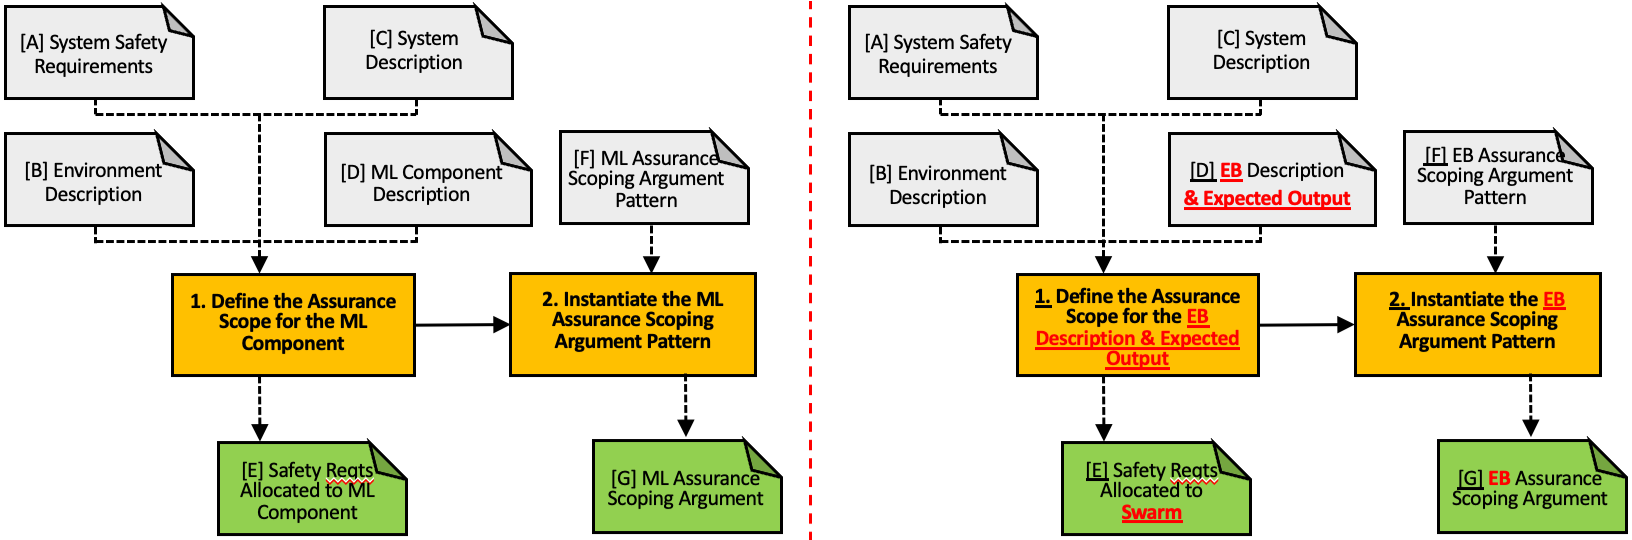
\includegraphics[width=1.0\textwidth]{figures/amlas-a-stage1.png}
%	\caption{Adapted AMLAS emergent behaviour assurance scoping process (right).}
%	\label{amlas-a-stage1}
%\end{figure*}

\begin{figure}[!h]
	\centering
	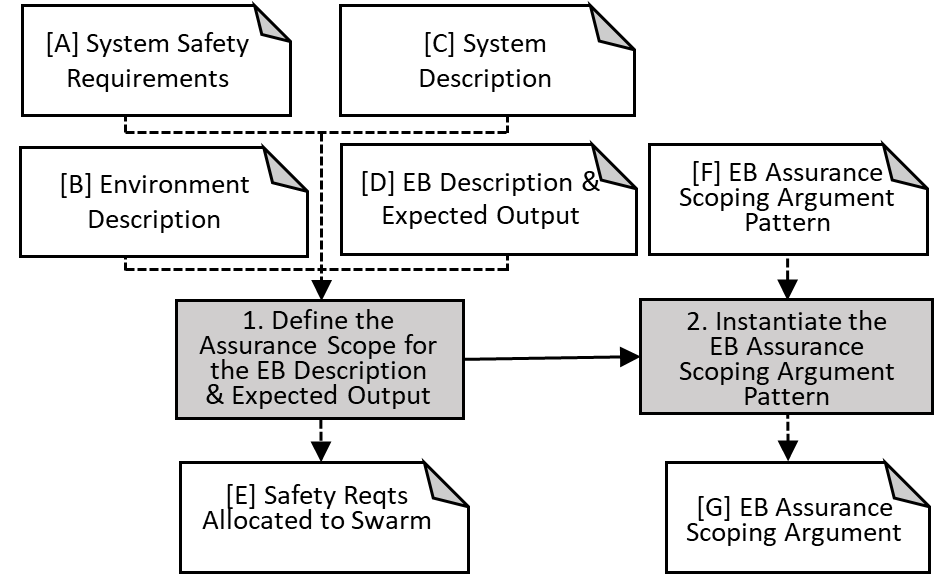
\includegraphics[width=0.5\textwidth]{figures/AMLAS-STAGE-1-V3.png}
	\caption{Stage 1: Adapted AMLAS emergent behaviour assurance scoping process.}
	\label{amlas-a-stage1}
\end{figure}

\subsection{Stage 1: EB Safety Assurance Scoping} \label{framework-stage1}
In this study, we look at inherent swarm qualities and the adaptation that arises from these qualities. 
In a swarm, individual robots execute simple behaviours or algorithms, and these simple behaviours when performed by a large number of agents build to form \emph{emergent behaviours} (EB). 
%These simple behaviours performed by large numbers of agents build to emergent behaviours.
%For this, we will look into developing individual behaviours which when combined create an adaptive emergence. 
The adaptivity provided by this emergence requires us to provide \textit{assurance} (e.g. safety assurance). 
At present, our study does not consider machine learning components of individual agents. Instead, these will be considered as part of future work once AMLAS has been applied to the swarm.
%However, we may consider this later once AMLAS has been applied to the swarm.

The adapted Stage 1 contains two activities which are performed to define the safety assurance scope for the swarm (see Fig.~\ref{amlas-a-stage1}). In activity 2 we use the artefacts generated from Stage 1 to instantiate the EB Assurance Scoping Argument Pattern, producing output [F] (Displayed in Fig.~\ref{stage1-ap}).

% \subsubsection*{Activity 1. Define the safety assurance scope for the EB description and expected output}
%\noindent \textbf{Activity 1: Define the safety assurance scope for the EB description and expected output}
The goal of activity 1 is to define the safety assurance scope for the EB description and expected output. The activity 1 requires the four following inputs: system safety requirements ([A]), the operating environment [B], the system description [C], and a description of the EB and expected output ([D]). 
Inputs A, B, C and D will later be used to determine the safety requirements which are allocated to the swarm. 
The requirements defined in Stage 1 are independent of any EB technique or metric. Instead, these requirements reflect the need for the swarm to perform safely with the system regardless of the deployed technology. The output of this activity is the safety requirements that are allocated to the swarm [E].

%\subsubsection*{Activity 6. Define Data Requirements}
%\paragraph*{[L.0] Data Type Requirements}
\paragraph*{[A] System Safety Requirements}
%\noindent \textbf{Artefact A -- System safety requirements: }
The system safety assessment process generates the safety requirements of the swarm, which covers identification of hazards and risk analysis. 
As illustrated in Fig.~\ref{failure-events}, this can be shown in the form of concrete failure conditions from an individual robot propagating through the swarm neighbourhood, resulting in swarm-level hazards. 
Although this has been illustrated as a simplified linear chain of events, in reality this represents a complex sequence which can be difficult to distil into distinct events and cause.

With respect to hazard identification and risk analysis performed in our study, in the \textit{cloakroom} use case, a key hazard is the blocking of critical paths. 
This can result in humans or other agents in the swarm unable to travel to urgent locations in a safe manner. In high risk use cases, such as wildfire detection, a considerable hazard can be presented should a critical fault go undetected. This can result in swarm operating with critically faulty agents resulting in the emergence of unsafe behaviour. The detection and labelling of faults does, however, require caution and a level of trade off. In the event of a misdiagnose of fault (for example, a minor fault being labelled as a critical fault e.g. a minor reduction of the wheel speed labelled as full motor failure), The system or user may end up removing key agents from the swarm who's fault is in fact not impact upon the emergent behaviour of the system. Such an occurrence would result in significant loss of performance and efficacy in the swarms task.

\begin{figure}[!t]
	\centering
	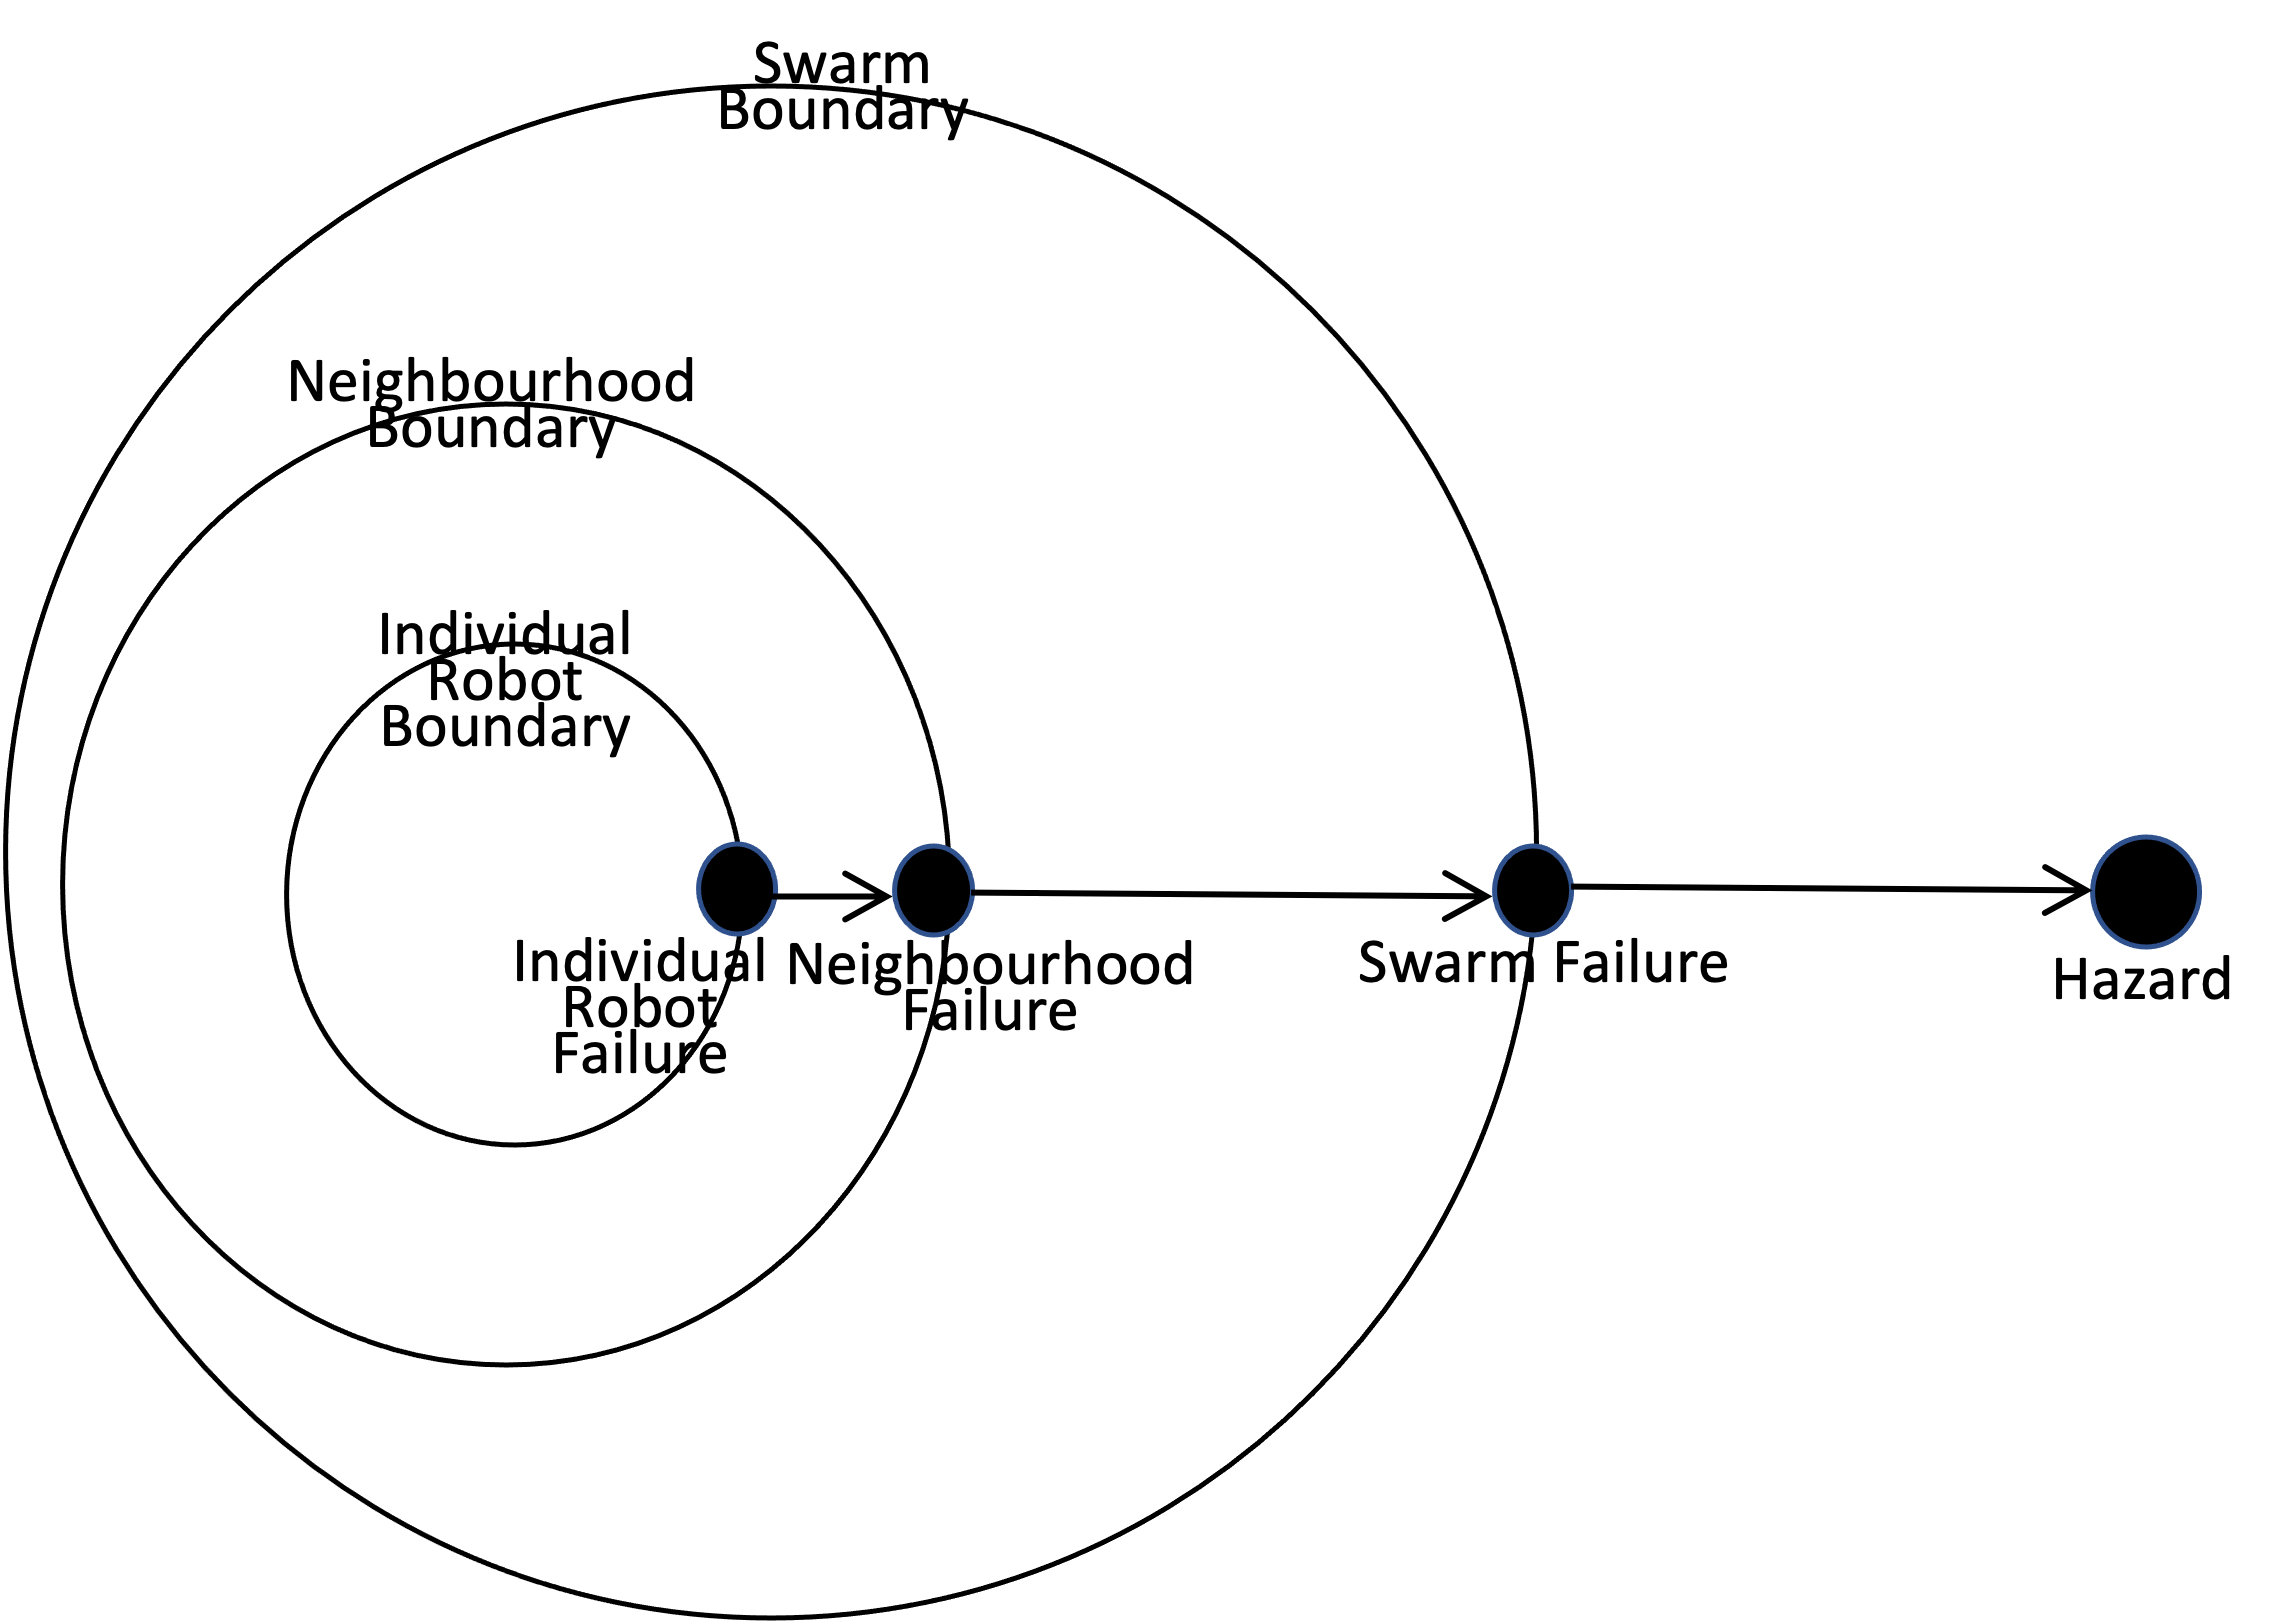
\includegraphics[width=0.5\textwidth]{figures/stage1-failureevents.png}
	\caption{Failure conditions in a swarm [adapted from DO-178C, AMLAS].}
	\label{failure-events}
\end{figure}
\paragraph*{[B] Environment Description}
%\noindent \textbf{Artefact B -- Environment description: }
As in AMLAS guidance, when allocating safety requirements to the swarm, it is essential to consider the system environment, which is represented by Artefact B. 
Based on the primary use case of our study, we can provide a description of their environments as follows:

\textit{A swarm of robotic agents collecting and delivering jackets, stored in small box-like containers within a cloakroom}. Agents are required to navigate a public space between collection and delivery points of jackets. Agents use local communication, perception, and data to form an emergent system of navigation that allows them to easily traverse the public space between jacket collection and delivery points.

% \textit{A swarm of UAVs monitoring wildfire risks in a natural environment}. Here, agents will be required to stay within communication range of each other, effectively covering the search area and accurately detecting risks of fire.

% \textit{Social swarm: brainstorming at an event}. Humans input their opinions on agents which then cluster based on the input. Humans follow the agent they interacted with and user groups emerge in the process.

\paragraph*{[C] System Description}
%\noindent \textbf{Artefact C -- System description: }
To describe our logistics use case, we must consider three inputs: sensor availability, neighbourhood data, and swarm parameters. 

In this instance, the \textit{sensors} available to agents might be: cameras, Bluetooth communication devices, and light detection \& ranging systems (see Fig.~\ref{system-description}). 

The neighbourhood data of the swarm can be specified through the communication systems available to agents, in this case Bluetooth. Through the use of the short range communication available to them, we can assume agents have access to neighbourhood data such as: the approximate position of local agents, current behaviour statuses, an approximate history of box movement, and the amount of time deployed. 

As for the swarm level parameters, we can consider options specified by a user i.e. the number of agents deployed, the maximum speed of agents, and the number of agents allowed to be active at a time.

Once we have defined these three inputs they are fed to the individual agents to instruct their behaviour. This behaviour, once enacted by the multiple agents, produces a swarm level emergence as the individuals interact with one another and their environment.

% \begin{figure}
% 	\centering
% 	
\includegraphics[width=0.4\textwidth]{figures/stage1-systema.png}
% 	\caption{System description.}
% 	\label{system-description}
% \end{figure}

\begin{figure}
\centering
\begin{minipage}{.5\textwidth}
    \centering
    
\includegraphics[width=0.95\textwidth]{figures/stage1-systema.png}
    \caption{System description.}
    \label{system-description}
\end{minipage}%
\begin{minipage}{.5\textwidth}
    \centering
    
\includegraphics[width=0.95\textwidth]{figures/stage1-argumentpattern-v2.png}
    \caption{EB Safety assurance scoping argument pattern.}
    \label{stage1-ap}
\end{minipage}
\end{figure}

\paragraph*{[D] EB Description and Expected Output}
%\noindent \textbf{Artefact D -- EB description and expected output: }
%This artefact describes the role and scope of the component within the system of which it is part, and the interfaces to which it is exposed.
By ``expected output", we refer to the gains that can arise from the system by deploying multiple agents. For our logistics use case, the output is a collaborative system capable of collecting, sorting and redelivering jackets in a public setting. 

To achieved this output, the emergent behaviour of the system needs to be manually engineered by a swarm engineer with consideration to the available sub-behaviours within an agent and the constraints outlined in the system description.

%\noindent \textbf{Activity 2: Instantiate the EB assurance scoping argument pattern}
%
%\noindent \textbf{Artefact F -- EB Safety assurance scoping argument pattern: }
% \subsubsection*{Activity 2: Instantiate the EB Assurance Scoping Argument Pattern}

% \paragraph*{Activity 2:}
% In activity 2 we look to instantiate the EB Assurance Scoping Argument Pattern, producing output [F] (Displayed in Fig.~\ref{stage1-ap}).

% \begin{figure}
% 	\centering
% 	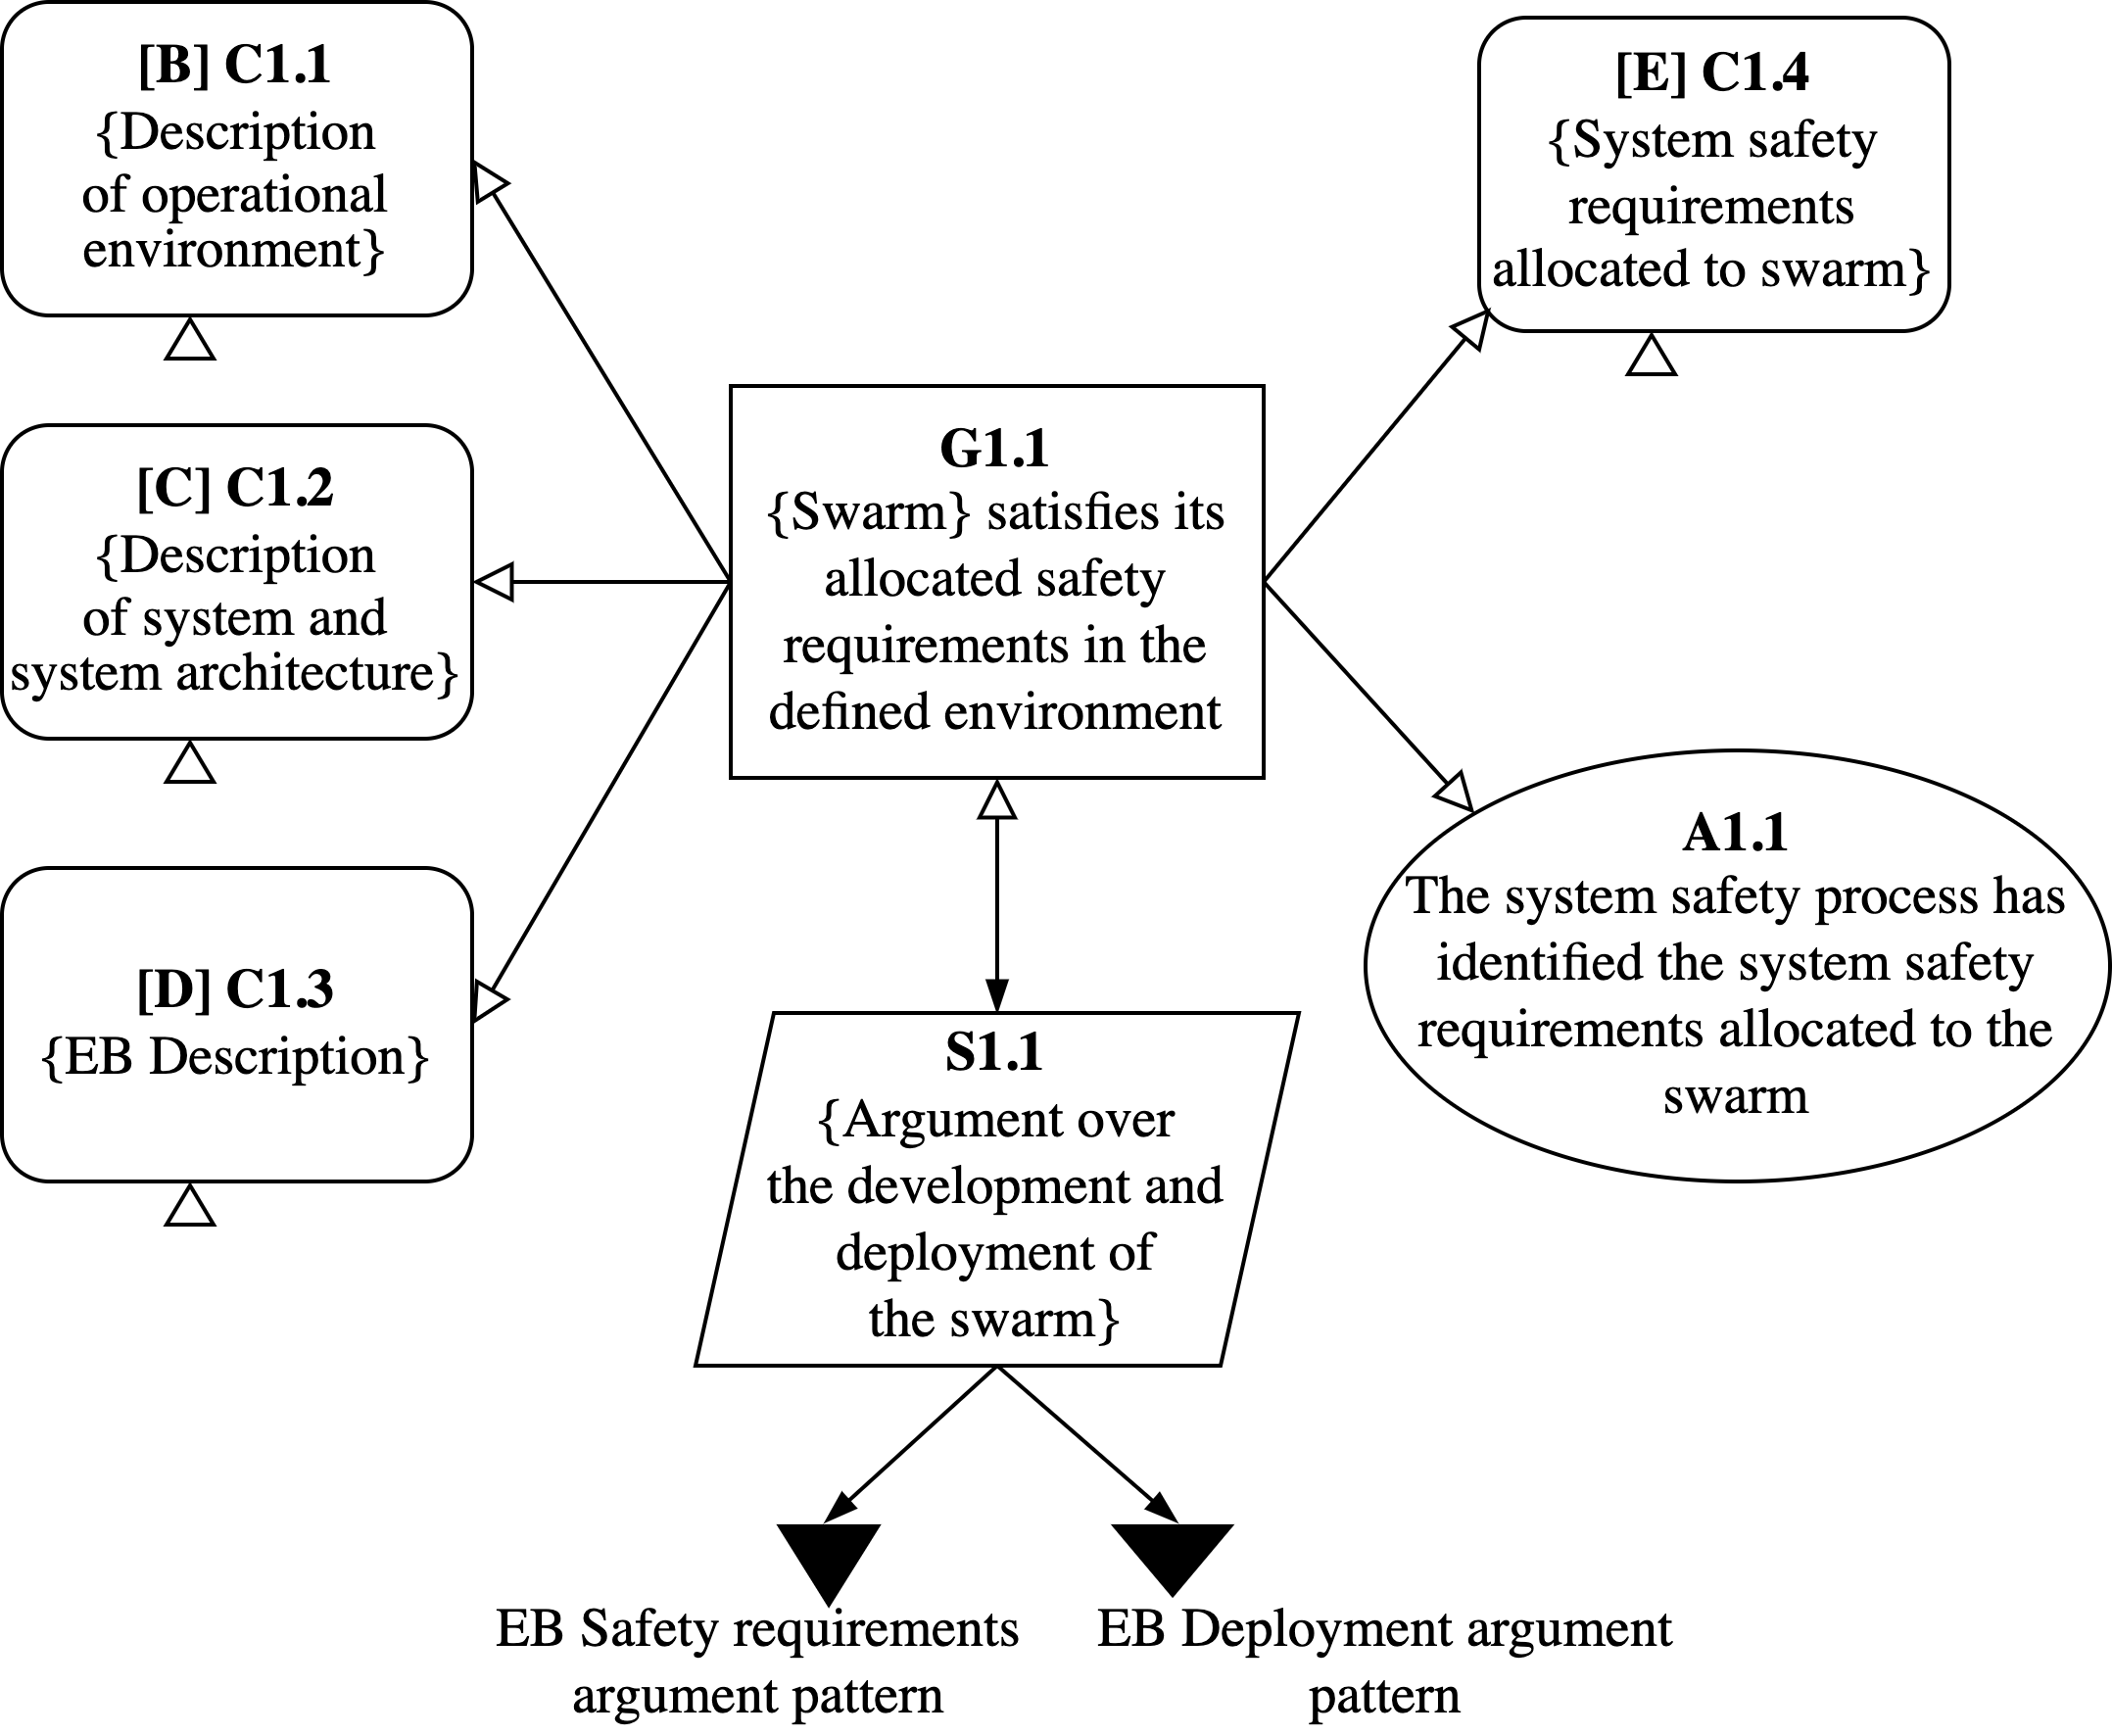
\includegraphics[width=0.4\textwidth]{figures/stage1-argumentpattern.png}
% 	\caption{EB Safety assurance scoping argument pattern.}
% 	\label{stage1-ap}
% \end{figure}

\subsection{Stage 2: EB Safety Requirements Assurance} \label{framework-stage2}
%\noindent \textbf{\textit{[Lead:  WP1; Other: WP2, WP3]}}\\ 
%\noindent\textbf{\textit{[Author Guidelines: total 7 pages (maximum); \\Format/structure: Describe adapted AMLAS activities, inputs and outputs using cloakroom case study examples. \\
		%\noindent WP1 = (Activities: 3, 4, 5; Inputs: E, I; Outputs: H, J, K: 2700 words / 3 pages maximum))\\
		%\noindent WP2 = (List of Ethical Requirements and Description: 1800 words / 2 pages maximum)\\
		%\noindent WP3 = (List of Socio-Technical/Regulatory Requirements and Description: 1800 words / 2 pages maximum)]
		%}}\\
As in AMLAS, adapted Stage 2 contains three activities (Fig.~\ref{amlas-a-stage2}), which are performed to provide assurance in EB safety requirements for the swarm. 
In activity 5, the artefacts generated are used to instantiate the EB safety requirements assurance argument pattern. The scope of this stage is limited to the EB model of the swarm.

\begin{figure}
\centering
\begin{minipage}{.5\textwidth}
    \centering
    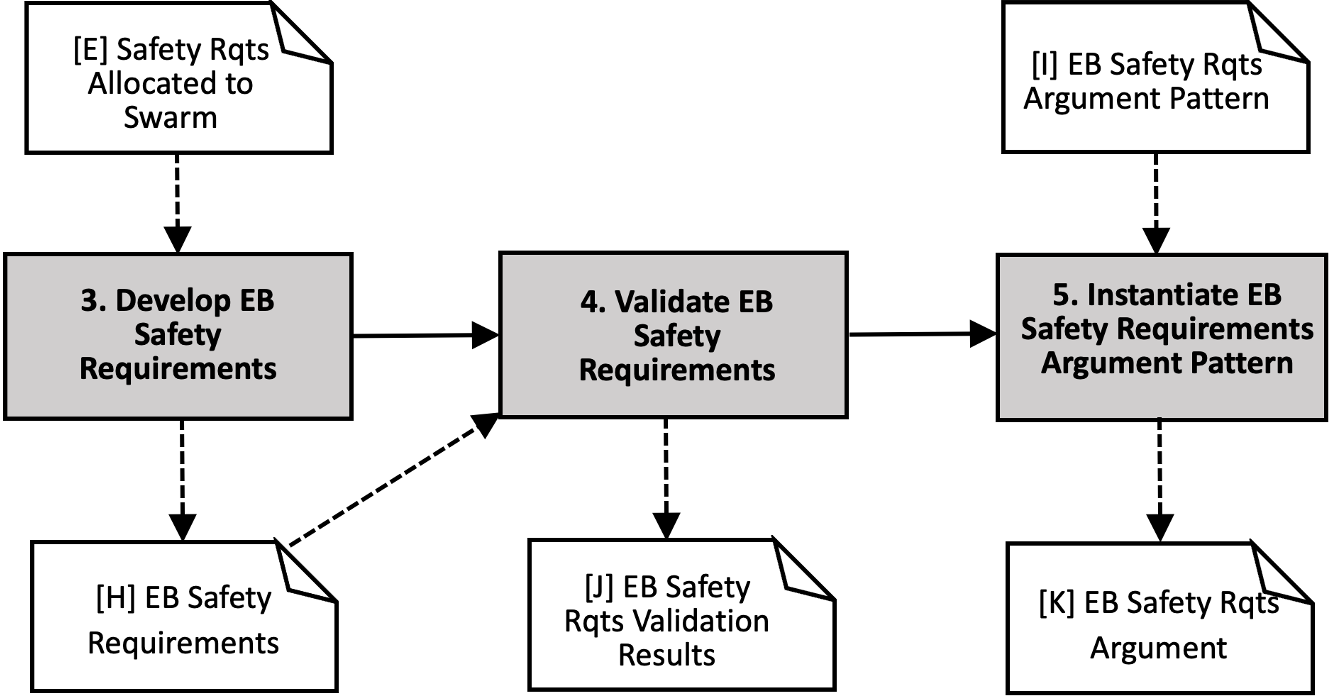
\includegraphics[trim={0mm -6mm 0mm -6mm},clip,width=\textwidth]{figures/amlas-a-stage2-v2.png}
    \caption{Stage 2: Adapted AMLAS emergent behaviour safety requirements assurance process.}
    \label{amlas-a-stage2}
\end{minipage}%
\begin{minipage}{.5\textwidth}
    \centering
    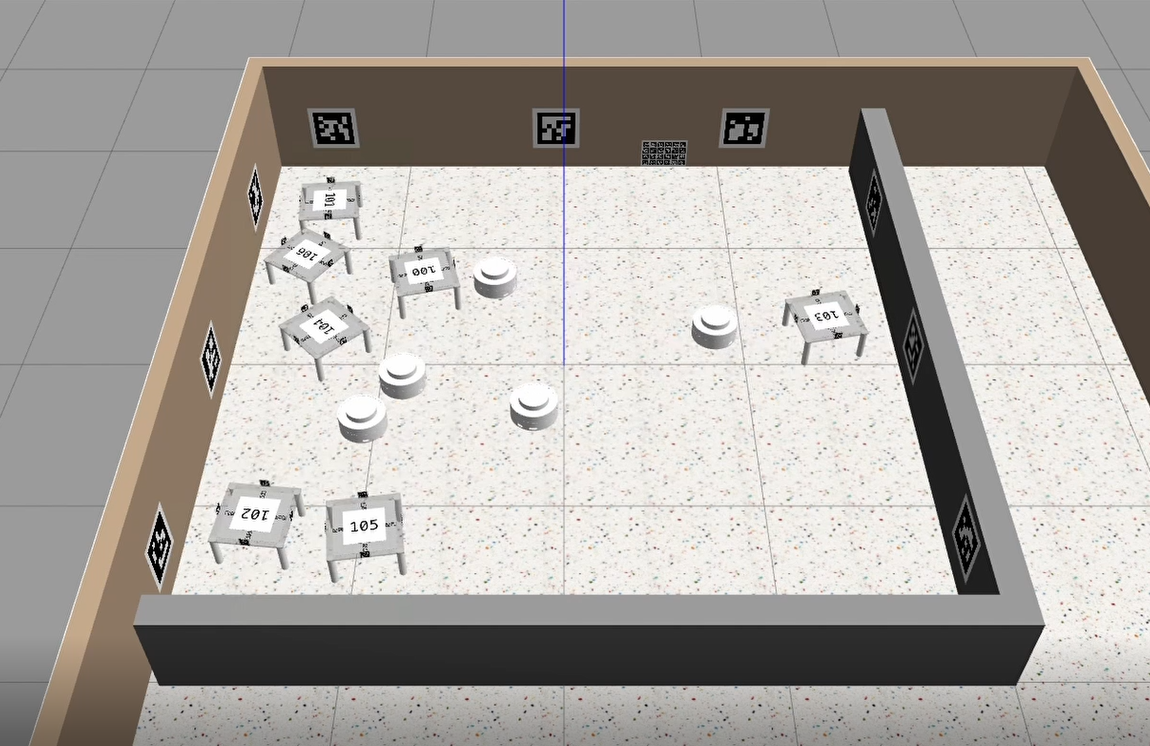
\includegraphics[trim={30mm 25mm 45mm 30mm},clip,width=0.9\textwidth]{figures/3Dsim.png}
    \caption{3D simulation created to validate several EB safety requirements of the cloakroom.}
    \label{3Dsim}
\end{minipage}
\end{figure}

% \begin{figure}[!t]
% 	\centering
% 	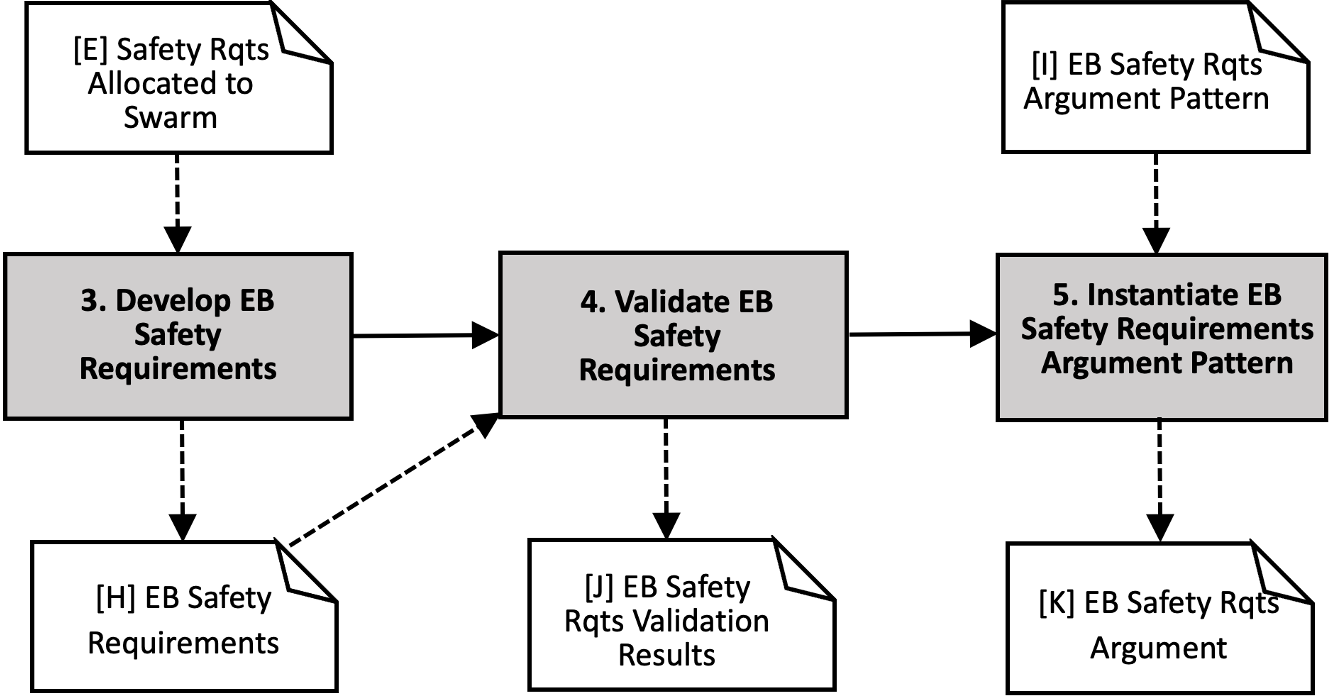
\includegraphics[width=0.5\textwidth]{figures/amlas-a-stage2-v2.png}
% 	\caption{Stage 2: Adapted AMLAS emergent behaviour safety requirements assurance process.}
% 	\label{amlas-a-stage2}
% \end{figure}

%\subsubsection*{Activity 6. Define Data Requirements}
\subsubsection*{Activity 3. Develop EB Safety Requirements}
%\noindent \textbf{Activity 3: Develop EB safety requirements}

The required input to Activity 3 in Stage 2 is the safety requirements allocated to the swarm ([E]).
We define EB safety requirements to control the risk of the swarm to system-level hazards by taking into account of the defined system architecture and operating environment. 

As in AMLAS, although there can be a wide range of requirements for the swarm like scalability, security and interpretability, the EB safety requirements need to be limited to the ones that have an impact on the operational safety of the system. 
Other types of requirements (e.g. security, scalability) need to be defined as EB safety requirements, only if their behaviours or underlying constraints have an influence on the safety-criticality of the swarm's output.  

The AMLAS guidance prescribes two types of requirements for ML components: performance and robustness. 
In the swarm context, we consider four types of requirements: \emph{performance}, \emph{adaptability}, \emph{human safety}, and \emph{environment}.
Robustness in the swarm context is a more broad notion, thus we introduce adaptability and environment sub-categories. 
In AMLAS, one key approach when defining robustness requirements is to consider the dimensions of variation which exist in the input space. In the swarms context, this can be variation in the simulation space instead of the input space. 

We consider several performance safety metrics under the four requirements categories: 
(i) performance: low impact and high impact collisions; 
(ii) adaptability: percentage of swarm stationary outside of the delivery site, number of stationary agents, time since last agent moved; 
(iii) human-safety: velocity or average velocity of agents, swarm size, rate of human encountered, proximity to humans;
(iv) environment: sum of objects/$m^2$.

For the performance, adaptability and human-safety requirements categories, we formulate requirements under three sub-categories: \emph{faultless operations}, \emph{failure modes (graceful degradation)}, and \emph{worst case}. 
In the conventional AMLAS framework, the level of faults one expect in a single ML system is low. However, in a swarm system, we expect it to have more faults, as there are more agents which are more difficult to monitor. 
As for \emph{graceful degradation}, we mean what is the acceptable level of faults, their impact, and how the system should react when those faults are introduced. 
Thirdly, we consider requirements for \emph{worst case}, which account for the least acceptable impact the system should experience and means of avoiding it. 

\subsubsection*{Activity 4: Validate EB Safety Requirements}
%\noindent \textbf{Activity 4: Validate EB safety requirements}

The required input to Activity 4 in Stage 2 is the safety requirements allocated to the swarm ([E]). As suggested in AMLAS guidance, we use reviews and simulations to validate the EB safety requirements.

Regarding reviews, the requirements derived for the cloakroom were also inspected by a safety-critical systems engineering expert to ensure that the specified EB safety requirements for the swarm will deliver its intended safe operation. This expert has a wide experience in topics related to aerospace, defence and transportation; and the safety of autonomous systems. % Previously, this expert had reviewed the CovidSim modelling, which was instrumental in settling the UK lock-down policy. 

With respect to simulation, we have validated several EB safety requirements (all performance, adaptability, and environment requirements except requirement RQ 3.5) of the cloakroom system using a 3D simulator (Gazebo). This simulation is an exact replication of the 4m x 4m lab environment used for hardware implementation (see Fig.~\ref{3Dsim}). 

% \begin{figure}[!t]
% 	\centering
% 	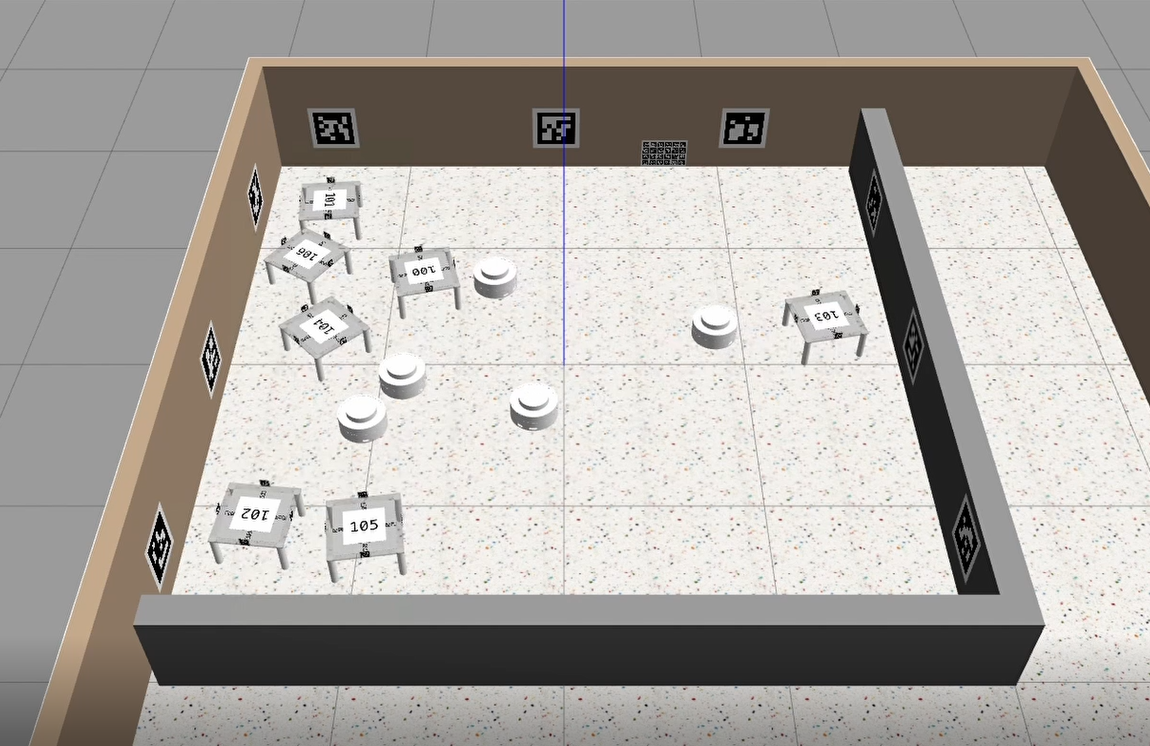
\includegraphics[width=0.5\textwidth]{figures/3Dsim.png}
% 	\caption{3D simulation created to validate several EB safety requirements of the cloakroom.}
% 	\label{3Dsim}
% \end{figure}

%\paragraph*{[H] EB Safety Requirements}
%\noindent \textbf{Stage 2 Requirements (Output H)}\\

From this activity we produce [H] EB Safety Requirements. These state the safety requirements relating to: Performance, Adaptability and Environment (examples shown in Table \ref{tab:reqs}). As well as Human safety requirements (examples shown in Table \ref{tab:human-s}).

% \begin{itemize}
% 	\item Performance requirements (see Table~\ref{tab:perormance}).
% 	\item Adaptability requirements (see Table~\ref{tab:adaptability}). Metric: Swarm waiting time/time-in-area.
% 	\item Human safety requirements (see Table~\ref{tab:human-s}). *Trained human in this case refers to workers within the case study setting. We assume that this individual has received relevant training \& experience in the use of the swarm system.
% 	\item Environmental specification (see Table~\ref{tab:environment}). *p$_o$ = sum of objects  / m$^2$
% \end{itemize}

\begin{table}[!t]
	\centering
	\begin{tabular}{p{5mm} p{116mm} }
            RQ & \textbf{Performance Requirements}\\
		\hline
		1.1 & The swarm \emph{shall} experience \textbf{$<$ 1 high impact (V $>$ 0.5m/s)} collisions across \textbf{a day} of faultless operation. \\ 
		\hline
		1.2 & The swarm \emph{shall} experience \textbf{$<$ 0.1\%} increase in \textbf{high impact} collisions across \textbf{a days} operation with \textbf{10\% injection} of \textbf{full communication fault} to the swarm.\\ 
		\hline
		1.3 & The swarm \emph{shall} experience \textbf{$<$ 0.1\%} increase in \textbf{high impact} collisions across \textbf{a days} operation with \textbf{50\% injection} of \textbf{half-of-wheels motor faults} to the swarm.	\\	
		\hline
		1.4 & The swarm \emph{shall} experience \textbf{$<$ 2 high impact (V $>$ 0.5m/s)} collisions across \textbf{a day} of faulty operation.  \\		[1ex] 		
		\hline
            & \textbf{Adaptability Requirements}\\
		\hline
		2.1 & The Swarm \emph{shall} have \textbf{$<$ 10\%} of its agents \textbf{stationary*} outside of the \textbf{delivery site} at a given time.
		*Assumption: Agents are considered stationary once they have not moved for $>$ 10 seconds.
		\\ 
		\hline
		2.2 & All agents of the swarm \emph{shall} move at least every \textbf{100 seconds} if outside of the \textbf{delivery site}. \\ 
		\hline
		2.3 & The swarm \emph{shall} experience $<$ 10\% increase in \textbf{number of stationary agents} at any given time with 50\% injection of half-of-wheels motor faults to the swarm. \\
		\hline
		2.4 & The swarm agents \emph{shall} experience $<$ 10\% increase in \textbf{stationary time} with 50\% injection of half-of-wheels motor faults to the swarm.\\ 
		\hline
		2.5 & The swarm \emph{shall} experience $<$ 10\% increase in \textbf{number of stationary agents} at any given time \textbf{10\% injection} of \textbf{full communication fault} to the swarm.\\
		\hline
		2.6 & The swarm agents \emph{shall} experience $<$ 10\% increase in \textbf{stationary time 10\% injection} of \textbf{full communication fault} to the swarm. \\	
		\hline
		2.7 & The Swarm \emph{shall} have \textbf{$<$ 20\%} of its agents \textbf{stationary*} outside of the \textbf{delivery site} at a given time.
		*Assumption: Agents are considered stationary once they have not moved for $>$ 10 seconds. \\
  		\hline
            & \textbf{Environmental Requirements}\\
		\hline
		3.1 & The swarm \emph{shall} perform as required in environmental density levels 0-4 \textbf{p$_o$* of objects (sum of boxes and agents)} in the environment.
		\\ 
		\hline
		3.2 & The swarm \emph{shall} perform as required when floor incline is 0-20 degrees.
		\\ 
		\hline
		3.3 & The swarm \emph{shall} perform as required in a dry environment.
		\\ 
		\hline
		3.4 & The swarm \emph{shall} perform as required in smooth-floored environments with step increases no greater than 0.5cm.
		\\ 
		\hline
		3.5 & The swarm \emph{shall} only operate in environments where humans have devices that identify the human’s whereabouts to the swarm agents.
		\\		[1ex] 		
		\hline
	\end{tabular}
	\caption{\label{tab:reqs}Safety rrequirements for the cloakroom.}
\end{table}

% \begin{table}[!t]
% 	\centering
% 	\begin{tabular}{|p{10mm}|p{112mm}|}
% 		\hline
% 		& \textbf{Requirements for Faultless Operations} \\
% 		\hline
% 		RQ1.1 & The swarm \emph{shall} experience \textbf{$<$ 1 low impact (V $<$ 0.5m/s)} collisions across \textbf{1000} seconds of faultless operation. \\ 
% 		\hline
% 		RQ1.2 & The swarm \emph{shall} experience \textbf{$<$ 1 high impact (V $>$ 0.5m/s)} collisions across \textbf{a day} of faultless operation. \\ 
% 		\hline
% 		& \textbf{Requirements for Failure Modes (Graceful Degradation): } \\
% 		\hline
% 		RQ1.3 & The swarm \emph{shall} experience \textbf{$<$ 10\%} increase in \textbf{low impact} collisions across \textbf{1000} seconds of operation with \textbf{10\% injection} of \textbf{full communication fault} to the swarm. \\
% 		\hline
% 		RQ1.4 & The swarm \emph{shall} experience \textbf{$<$ 0.1\%} increase in \textbf{high impact} collisions across \textbf{a days} operation with \textbf{10\% injection} of \textbf{full communication fault} to the swarm.\\ 
% 		\hline
% 		RQ1.5 & The swarm \emph{shall} experience \textbf{$<$ 10\%} increase in \textbf{low impact} collisions across \textbf{1000} seconds of operation with \textbf{50\% injection} of \textbf{half-of-wheels motor faults} to the swarm.\\
% 		\hline
% 		RQ1.6 & The swarm \emph{shall} experience \textbf{$<$ 0.1\%} increase in \textbf{high impact} collisions across \textbf{a days} operation with \textbf{50\% injection} of \textbf{half-of-wheels motor faults} to the swarm.	\\	
% 		\hline
% 		& \textbf{Requirements for Worst Case: } \\
% 		\hline
% 		RQ1.7 & The swarm \emph{shall} experience \textbf{$<$ 2 low impact (V $<$ 0.5m/s)} collisions across \textbf{1000} seconds of faulty operation. \\			\hline	
% 		RQ1.8 & The swarm \emph{shall} experience \textbf{$<$ 2 high impact (V $>$ 0.5m/s)} collisions across \textbf{a day} of faulty operation.  \\		[1ex] 		
% 		\hline
% 	\end{tabular}
% 	\caption{\label{tab:perormance}Performance requirements for the cloakroom.}
% \end{table}    

% \begin{table}[!t]
% 	\centering
% 	\begin{tabular}{|p{10mm}|p{112mm}|}
% 		\hline
% 		& \textbf{Requirements for Faultless Operations} \\
% 		\hline
% 		RQ2.1 & The Swarm \emph{shall} have \textbf{$<$ 10\%} of its agents \textbf{stationary*} outside of the \textbf{delivery site} at a given time.
% 		*Assumption: Agents are considered stationary once they have not moved for $>$ 10 seconds.
% 		\\ 
% 		\hline
% 		RQ2.2 & All agents of the swarm \emph{shall} move at least every \textbf{100 seconds} if outside of the \textbf{delivery site}. \\ 
% 		\hline
% 		& \textbf{Requirements for Failure Modes (Graceful Degradation): } \\
% 		\hline
% 		RQ2.3 & The swarm \emph{shall} experience $<$ 10\% increase in \textbf{number of stationary agents} at any given time with 50\% injection of half-of-wheels motor faults to the swarm. \\
% 		\hline
% 		RQ2.4 & The swarm agents \emph{shall} experience $<$ 10\% increase in \textbf{stationary time} with 50\% injection of half-of-wheels motor faults to the swarm.\\ 
% 		\hline
% 		RQ2.5 & The swarm \emph{shall} experience $<$ 10\% increase in \textbf{number of stationary agents} at any given time \textbf{10\% injection} of \textbf{full communication fault} to the swarm.\\
% 		\hline
% 		RQ2.6 & The swarm agents \emph{shall} experience $<$ 10\% increase in \textbf{stationary time 10\% injection} of \textbf{full communication fault} to the swarm. \\	
% 		\hline
% 		& \textbf{Requirements for Worst Case: } \\
% 		\hline
% 		RQ2.7 & The Swarm \emph{shall} have \textbf{$<$ 20\%} of its agents \textbf{stationary*} outside of the \textbf{delivery site} at a given time.
% 		*Assumption: Agents are considered stationary once they have not moved for $>$ 10 seconds. \\			\hline	
% 		RQ2.8 & All agents of the swarm \emph{shall} move at least every \textbf{200 seconds} if outside of the \textbf{delivery site}.\\		[1ex] 		
% 		\hline
% 	\end{tabular}
% 	\caption{\label{tab:adaptability}Adaptability requirements for the cloakroom.}
% \end{table}   



\begin{table}[!h]
	\centering
	\begin{tabular}{p{6mm} p{116mm}}
		RQ & \textbf{Human Safety Requirements} \\
		\hline
		4.1 & The agents in the swarm \emph{shall} travel at speeds of less than \textbf{0.5m/s} when within \textbf{2m} distance of a \textbf{trained human*.}
		\\ 
		\hline
	    4.2 & The agents in the swarm \emph{shall} travel at speeds of less than \textbf{0.25m/s} when within \textbf{3m} distance of a \textbf{member of the public}.
		\\ 
		\hline
		4.3 & The agents in the swarm \emph{shall} only come within \textbf{2m} distance of a \textbf{human $<$ 10} times collectively across \textbf{1000 seconds} of \textbf{faultless} operations.
		\\ 
		\hline
		4.4 & The swarm \emph{shall} only allow \textbf{$<$ 5 agents} to request intervention from a \textbf{trained human*} at a given time
		\\ 
		\hline
		4.5 & A Trained human \emph{shall} monitor 5-20 agents at a given time.
		\\ 
		\hline
		4.6 & The swarm \emph{shall} only allow \textbf{1 agent} to request input from a \textbf{member of the public} at a given time.
		\\ 
		\hline
		4.7 & A member of the public \emph{shall} receive $<$ 5 agents of swarm information at a given time.
		\\ 
		\hline
		4.8 & The swarm \emph{shall} experience \textbf{$<$ 10\%} increase in \textbf{human encounters} across 1000 seconds of operation with \textbf{10\% injection} of \textbf{full communication fault} to the swarm. \\
		\hline
		4.9 & The swarm \emph{shall} experience \textbf{$<$ 10\%} increase in \textbf{human encounters }across 1000 seconds of operation with \textbf{50\% injection} of \textbf{half-of-wheels motor faults} to the swarm.\\
		\hline
		4.10 & The agents in the swarm \emph{shall} only come within \textbf{2m} distance of a \textbf{human $<$ 20} times collectively across \textbf{1000 seconds} of \textbf{faulty} operations.
		\\		[1ex] 		
		\hline
	\end{tabular}
	\caption{\label{tab:human-s}Human safety requirements for the cloakroom.}
\end{table}   


% \begin{table}[!h]
% 	\centering
% 	\begin{tabular}{|p{10mm}|p{112mm}|}
% 		\hline
% 		RQ4.1 & The swarm \emph{shall} perform as required in environmental density levels 0-4 \textbf{p$_o$* of objects (sum of boxes and agents)} in the environment.
% 		\\ 
% 		\hline
% 		RQ4.2 & The swarm \emph{shall} perform as required when floor incline is 0-20 degrees.
% 		\\ 
% 		\hline
% 		RQ4.3 & The swarm \emph{shall} perform as required in a dry environment.
% 		\\ 
% 		\hline
% 		RQ4.4 & The swarm \emph{shall} perform as required in smooth-floored environments with step increases no greater than 0.5cm.
% 		\\ 
% 		\hline
% 		RQ4.5 & The swarm \emph{shall} only operate in environments where humans have devices that identify the human’s whereabouts to the swarm agents.
% 		\\		[1ex] 		
% 		\hline
% 	\end{tabular}
% 	\caption{\label{tab:environment}Environment requirements for the cloakroom.}
% \end{table}   

\begin{table}[!h]
	\centering
	\begin{tabular}{|p{9.6cm}| p{6mm}| p{6mm}| p{6mm}| p{4mm}| p{4mm}|} %{|*{18}{c|}}  % repeats {c|} 18 times 
		\hline
		\multicolumn{6}{|p{12.2cm}|}{\textbf{System: Cloakroom System} \newline \textbf{Specifier: Safety Engineer} \newline \textbf{Date: 03 October 2022} \newline The cloakroom system requires a high degree of transparency for the trained workers, but with less transparency for the customers, due to concerns of exploitation.} \\ \hline
		\multirow{2}{12.2cm}{\textbf{IEEE Std 7001-2021 subclause \newline (C = cumulative, NC = non cumulative)}} & \multicolumn{5}{p{5mm}|}{\textbf{Levels}} \\ \cline{2-6}
		& 1 & 2 & 3 & 4 & 5 \\ \hline
		5.1.1 Users (NC) & $X^*$ & $X^*$ & & & \\ & $X^{**}$ & $X^{**}$ & $X^{**}$ & & \\ \hline
		\multicolumn{6}{|p{12.2cm}|}{Note- Two categories of users are defined as follows: \newline
			* \textit{Customers} who are non-expert users.\newline %Transparency is comparatively more important to this category compared to trained staff.
			** \textit{Trained staff} are expert or super users of the cloakroom.} \\  \hline
		5.1.2 General public and bystanders (NC) & X & X & & & \\ \hline
		\multicolumn{6}{|p{12.2cm}|}{NOTE—The individual robots in the swarm are clearly identified as robots, with warnings; they are fitted with cameras for navigation, with limited views so that they do not collect personal data. This group is only indirectly affected by the system. }\\ \hline
		5.2.1 Validation and certification agencies (C) & X & X & & & \\ \hline
		\multicolumn{6}{|p{12.2cm}|}{NOTE—Evidence of validation and certification to a lower degree is sufficient such as equipped with a data-logging system, given the less-sensitivity of the system.}\\ \hline
		5.2.2 Incident investigators (C) & X & X & & & \\ \hline
		\multicolumn{6}{|p{12.2cm}|}{NOTE—The cloakroom system must log all events securely to support incident investigations, noting that incident investigation may be triggered by a customer, or a watchdog raising concerns about the functions of the swarm. The agents in the swarm are equipped with a data logging system that records high level decisions (no personal data will be recorded). Levels 3--5 are not considered essential, as the agents in the swarm will only require a limited number of behaviours (with no learning).  }\\ \hline
		5.2.3 Expert advisors in administrative actions or litigation (NC) & X & & & & \\ \hline
		\multicolumn{6}{|p{12.2cm}|}{NOTE—The company should take into account ISO 9001 accreditation or equivalent for the swarm.}\\ \hline
	\end{tabular}
	\caption{\label{tab:transparency}Transparency requirements for the cloakroom: System transparency specification.}
 % These can be deployers and administrators of the swarm, such as site managers. They require a medium level of understanding of how the swarm works, including the ability to ask an agent to explain its decisions, to predict the system's behaviour in a given situation and repair simple faults of agents.
\end{table}

%\paragraph*{Transparency Requirements: System Transparency Specification}\label{transparency-r}
In addition to the safety requirements formulated based on AMLAS, we also formulate requirements for transparency. By using the IEEE P7001 standard we can specify transparency requirements for the cloakroom use case (outlined in Section \ref{ex:cloakroom}) prior to its implementation, which is known as a process of \textit{System Transparency Specification} (STS) \cite{IEEE-P7001}. IEEE P7001 describes a set of normative requirements on transparency and explainability, which must be satisfied to be labelled as compliant. % cite both
The score sheet summarizing the outcomes of the assessment is shown in Table~\ref{tab:transparency}. \\\\

% \subsubsection{Ethics Requirements}\label{ethics-r}
% Building on \cite{Porter2022}, and adapting it for our purposes, we developed ethics requirements for swarm robots around the ethical principles of beneficence, non-maleficence, respect for autonomy, and justice. To limit the scope of this paper, we decided to focus on the impact of our case study on members of the public, trained humans, manufacturers, and the company deploying the swarm, hence leaving aside questions about broader societal and environmental implications.

% The main ethics requirements, each corresponding to a principle, are shown in Table \ref{tab:ethics} below. 
% \begin{table}[!h]
% 	\centering
% 	\begin{tabular}{|p{10mm}|p{112mm}|}
% 		\hline
% 		& \textbf{ Ethics Requirements} \\
% 		\hline
% 		RQ1 & The swarm \textit{shall} provide benefits to stakeholders. \\ 
% 		\hline
% 		RQ2 & The swarm \textit{shall} avoid causing unjustified harm to stakeholders. \\ 
% 		\hline
% 		RQ3 & The swarm \textit{shall} avoid undue constraints on stakeholders' personal autonomy. \\
% 		\hline
% 		RQ4 & The swarm \textit{shall} allow fair treatment of stakeholders.  \\		[1ex] 		
% 		\hline
% 	\end{tabular}
% 	\caption{\label{tab:ethics}Ethics requirements for the cloakroom.}
% \end{table}  

% These broad requirements should be further specified, and this is where developing ethics matrices is helpful. The matrices allow us to identify benefits, risks of harm, and threats to autonomy and fair treatment caused by the development and deployment of the system. The significance and likelihood of the identified benefits, harms, and threats should then be considered to decide which can be tolerated and which should be addressed; for the latter, ethics sub-requirements should be developed to make changes to the design of the system, and so ensure the development of a more ethically aligned technology. Deciding which changes to prioritise is the most difficult part of the process, because there is no formulaic approach to follow; rather, this process requires interdisciplinary and multi-stakeholder discussions, individual and collective judgment, and ethics deliberation, which should include consideration of opportunity costs. However, that extends beyond the scope of this paper. Below we only give examples of how the matrices could be used to develop sub-requirements to specify RQ1-4. In line with the core aim of this paper, we only give examples focusing on the swarm's emergent behaviour.

% BEGINING OF PETE'S ADDITION

% \subsubsection{Using the Structural, Organisational, Technological, Epistemic, and Cultural (SOTEC) framework for a regulatory requirements analysis of autonomous robotic swarms}\label{regulations-r}

% In addition to ethical requirements, we also introduce regulatory requirements into the consideration of specification produced in stage 2.
% In particular we have observed the work of Macrae \cite{macrae2021learning}, who proposes: Structural, Organisational, Technological, Epistemic, and Cultural (SOTEC) framework of sociotechnical risk in Autonomous and Intelligent systems (AIS) and discusses its regulatory implications for autonomous swarms in a cloakroom scenario. The SOTEC framework proposes that risk and failure in AIS be understood in terms of five broad sociotechnical categories, each corresponding to different organisational, contextual, and human factors that might inform AIS safety requirements. The spotlight on sociotechnical sources of risk in AIS throughout section one provides a crucial launching point for the identification of regulatory requirements. Viewing regulatory requirement analysis from a sociotechnical perspective allows us to move away from a purely technical conception of requirements, and helps us design autonomous systems that better fit the organisation and operators’ work in which safety considerations are meaningful within the wider system and operational context. Based on these considerations, we illustrate the relevance of the SOTEC framework for crafting regulatory requirements for autonomous robotic swarms as a safety assurance mechanism. Following this, we then apply the framework by utilising insights from swarm engineers who are in the process of developing a case study of a swarm system for a cloakroom setting that is in early development and offering autonomous solutions to customers depositing their garments.

% END OF PETE'S ADDITIONS

\subsection{Stage 3: Data Management} \label{framework-stage3}
% \noindent \textbf{\textit{[Lead:  WP5]}}\\ 
% \noindent\textbf{\textit{Author Guidelines: 900–1800 words / 1–2 pages (maximum); \\Format/structure: Describe adapted AMLAS activities, inputs and outputs using cloakroom case study examples. Activities: 6, 7, 8; Inputs: H; Outputs: L0, L1, M, N, O, P, Q, S}}\\
% See Fig.~\ref{amlas-a-stage3}
% \begin{figure*}
% 	\centering
% 	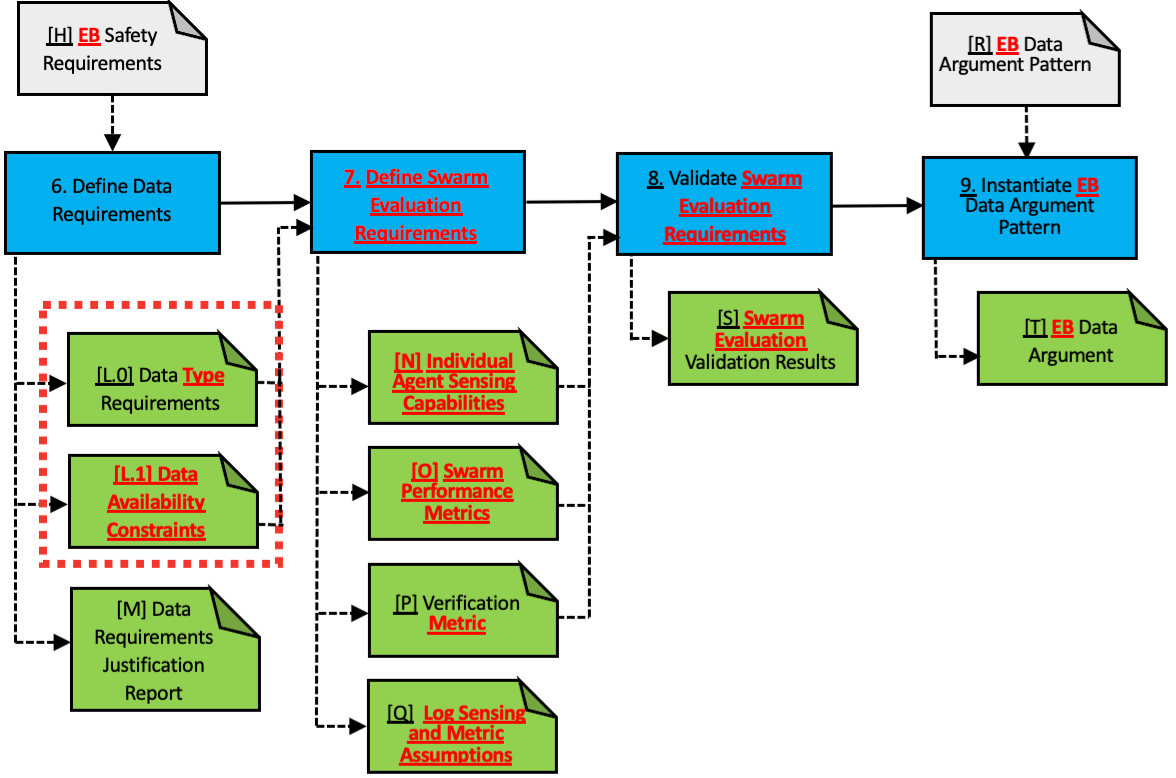
\includegraphics[width=1.0\textwidth]{figures/amlas-a-stage3.png}
% 	\caption{Adapted AMLAS data management process.}
% 	\label{amlas-a-stage3}
% \end{figure*}

When designing emergent behaviours data plays a vital role, though one that differs from the machine learning applications AMLAS was initially designed for. In order to address this difference, the following activities and outputs have been adjusted to take into account the swarm behavioural design process and the added complexities that come with multiple agents interacting with one another.

\begin{figure*}
	\centering
	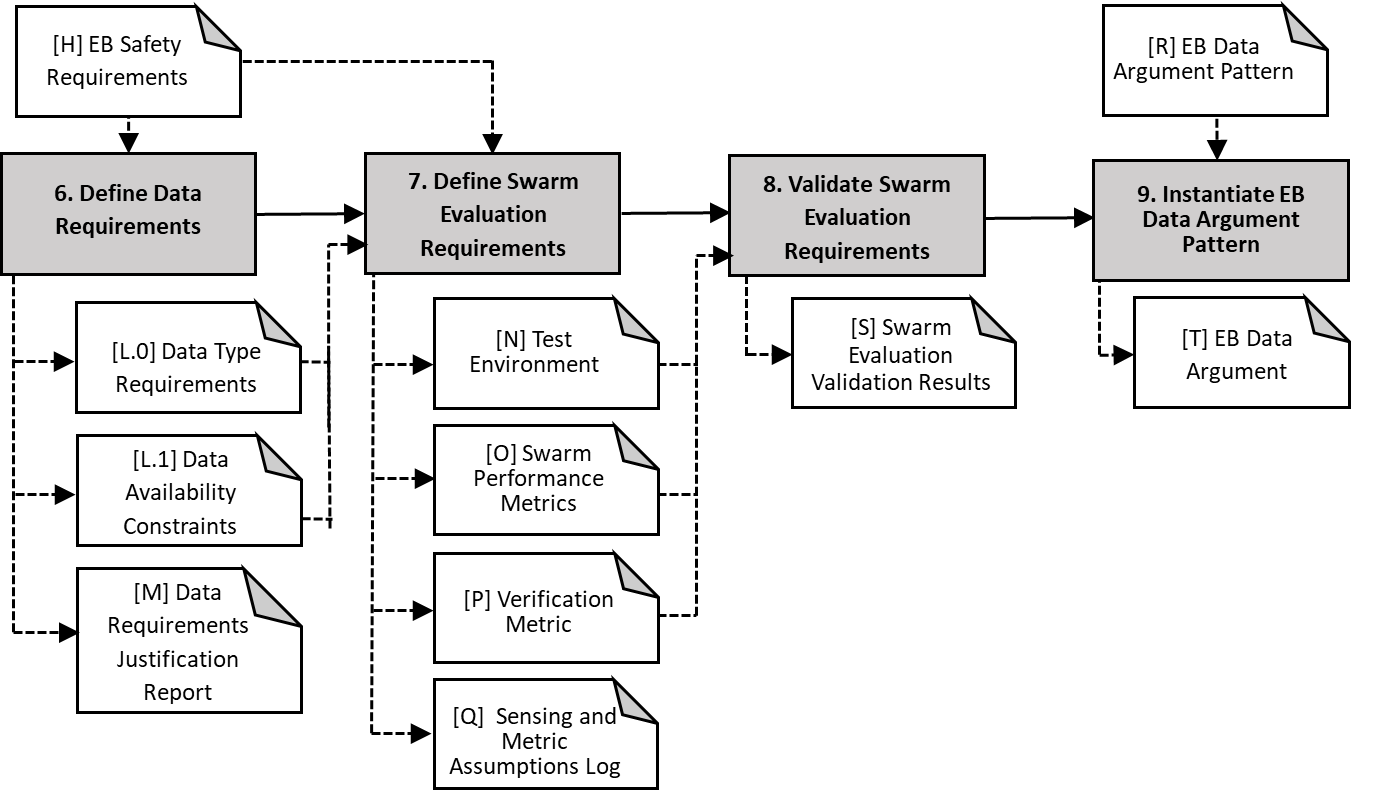
\includegraphics[width=0.8\textwidth]{figures/AMLAS-STAGE-3-V3.png}
	\caption{Adapted AMLAS data management process.}
	\label{amlas-a-stage3}
\end{figure*}

\subsubsection*{Activity 6. Define Data Requirements}

% AMLAS - This activity requires as input the ML safety requirements ([H]) as described in Stage 2 and, from these requirements, data requirements ([L]) shall be generated. Of particular interest in the development of data requirements are those safety requirements which pertain to the description of the system environment.

In our adaptation of activity 6 we take the emergent behaviour safety requirements [H] outlined in Stage 2 as an input (see Fig.~\ref{amlas-a-stage3}). These safety requirements guide the data requirements in this activity, feeding into the data specification that we outline here. Unlike the original AMLAS framework, we have split the data requirement [L] into two multi-agent focused requirements: [L.0] data type requirements and [L.1] data availability constraints.

% \begin{table}[!t]%[h]
%     \centering
%     \begin{tabular}{p{1cm} p{11cm}}
%         \textbf{ID} & \textbf{Example} \\
%         \hline
%         RQ 5.1 & All simulations shall include environments with different ranges of incline between 0-20\textdegree.\\
%         \hline
%         RQ 5.2 & All simulations shall be conducted in a dry environment.\\
%         \hline
%         RQ 5.3 & All simulations shall include floors with step increases that are $\leq$ 0.5 cm.\\
%     \end{tabular}
%     \caption{Relevance requirement examples for output [L.0].}
%     \label{tab:L0_relevance}
% \end{table}

\begin{table}[!t]%[h]
    \centering
    \begin{tabular}{p{0.6cm} p{11.6cm}}
        \textbf{RQ} & \textbf{Relevance Requirements Examples} \\
        \hline
        5.1 & All simulations shall include environments with ranges of incline between 0-20\textdegree.\\
        \hline
        5.2 & All simulations shall be conducted in a dry environment.\\
        % \hline
        % 5.3 & All simulations shall include floors with step increases that are $\leq$ 0.5 cm.\\
        \hline
         & \textbf{Completeness Requirements Examples} \\
        \hline
        6.1 & All simulations shall be repeated to include fault injections representative of full communication faults.\\
        \hline
        6.2 & All simulations shall be repeated a sufficient number of times to ensure results are representative of typical use.\\
        \hline
        6.3 & All simulations shall be repeated in multiple environments representative of those expected in real-world use of the system.\\
        % \hline
        % 6.4 & All simulations shall include sufficient range of robot density levels within the scope of the operational domain.\\ 
        \hline
         & \textbf{Accuracy Requirements Examples} \\
        \hline
        7.1 & All boxes shall only be considered `delivered’, if all four of the boxes’ feet are positioned within the delivery zone.\\
        \hline
        7.2 & All boxes shall only be considered `delivered’, once they are no longer in direct contact with a swarm agent.\\
        \hline
         & \textbf{Balance Requirements Examples} \\
        \hline
        8.1 & All simulations shall be repeated so as to obtain representative evaluations for each possible mode of failure (defined under performance, adaptability and human-safety requirements in Stage 2).\\
        \hline
        8.2 & All simulations shall be repeated equally across all test environments.\\
        \hline
    \end{tabular}
    \caption{Requirement examples for output [L.0].}
    \label{tab:L0_req}
\end{table}

\paragraph*{[L.0] Data Type Requirements}

This elements focus on the relevance, completeness, accuracy, and balance of the information that will be used to construct the swarm behaviour and will be subsequently used to test the emergent behaviour of the system prior to its deployment. 

The relevance of the data used in the development of the emergent behaviour specifies the extent to which the test environment must match the intended operating domain into which the model is to be deployed.

The completeness of the data specifies the conditions under which we test the behaviour algorithm i.e. the volume of experiments or tests that will be run, the variety of tests executed, and the diversity of environments expected to be used in the testing process. 

Accuracy in this context relates to the parameters defining the performance of the swarm systems primary function. For example, what constitutes a delivery in a logistics scenario, or under what conditions would an area be considered explored in a surveying mission. 

Balance, outside of a machine learning use case, refers the balance of the trials executed in the testing process of the emergent behaviour algorithm. By considering balance, we expect the number of tests conducted for failure modes or environments to be justified, ensuring that there is not an unrealistic bias in testing towards a particular scenario. We list examples of data requirements relating to relevance, completeness, accuracy, and balance in Table \ref{tab:L0_req}.

% \begin{table}%[h]
%     \centering
%     \begin{tabular}{p{1cm} p{11cm}}
%         \textbf{ID} & \textbf{Example} \\
%         \hline
%         RQ 6.1 & All simulations shall be repeated to include fault injections representative of full communication faults.\\
%         \hline
%         RQ 6.2 & All simulations shall be repeated a sufficient number of times to ensure results are representative of typical use.\\
%         \hline
%         RQ 6.3 & All simulations shall be repeated in multiple environments representative of those expected in real-world use of the system.\\
%         \hline
%         RQ 6.4 & All simulations shall include sufficient range of robot density levels within the scope of the operational domain.\\ 
%     \end{tabular}
%     \caption{Completeness requirement examples for output [L.0].}
%     \label{tab:L0_completeness}
% \end{table}



% \begin{table}[!t]
%     \centering
%     \begin{tabular}{p{1cm} p{11cm}}
%         \textbf{ID} & \textbf{Example} \\
%         \hline
%         RQ 7.1 & All boxes shall only be considered `delivered’, if all four of the boxes’ feet are positioned within the delivery zone.\\
%         \hline
%         RQ 7.2 & All boxes shall only be considered `delivered’, once they are no longer in direct contact with a swarm agent.\\
%     \end{tabular}
%     \caption{Accuracy requirement examples for output [L.0].}
%     \label{tab:L0_accuracy}
% \end{table}

% \begin{table}%[h]
%     \centering
%     \begin{tabular}{p{1cm} p{11cm}}
%         \textbf{ID} & \textbf{Example} \\
%         \hline
%         RQ 8.1 & All simulations shall be repeated so as to obtain representative evaluations for each possible mode of failure (defined under performance, adaptability and human-safety requirements in Stage 2).\\
%         \hline
%         RQ 8.2 & All simulations shall be repeated equally across all test environments.\\
%         \hline
%     \end{tabular}
%     \caption{Balance requirement examples for output [L.0].}
%     \label{tab:L0_balance}
% \end{table}

%In Table \ref{tab:L0} we list each of the requirement focuses considered in this output and provide respective examples of swarm data requirements.

% \begin{table}[H]
%     \centering
%     \begin{tabular}{p{2cm} p{6cm}}
%         \textbf{Requirement} & \textbf{Example} \\
%         \hline
%         Relevance & All simulations shall include environments with different ranges of incline between 0-20\textdegree.\\
%         \hline
%         & All simulations shall be conducted in a dry environment.\\
%         \hline
%         & All simulations shall include floors with step increases that are \leq 0.5 cm.\\
%         \hline
%         Completeness & All simulations shall be repeated to include fault injections representative of full communication faults.\\
%         \hline
%         & All simulations shall be repeated a sufficient number of times to ensure results are representative of typical use.\\
%         \hline
%         & All simulations shall be repeated in multiple environments representative of those expected in real-world use of the system.\\
%         \hline
%         & All simulations shall include sufficient range of robot density levels within the scope of the operational domain.\\
%         \hline
%         Accuracy & All boxes shall only be considered `delivered’, if all four of the boxes’ feet are positioned within the delivery zone.\\
%         \hline
%         & All boxes shall only be considered `delivered’, once they are no longer in direct contact with a swarm agent.\\
%         \hline
%         Balance & All simulations shall be repeated equally across all test environments.\\
%         \hline
%         & All simulations shall be repeated equally across all test environments.\\
%     \end{tabular}
%     \caption{Requirement focuses for output [L.0] with representative examples from the cloakroom use case.}
%     \label{tab:L0}
% \end{table}
\paragraph*{[L.1] Data Availability Constraints}
With the introduction of multiple agents comes the issue of data availability. Distributed communication is a key feature found in emergent systems. As such, it is crucial to define how much information each agent is expected to hold, how easily data may transfer between agents, and across what range agents should be able to transfer information between one another. Feasible constraints include:


\textit{Storage capacity: }The swarm agents shall have a maximum of 2 GB of information stored on board at any point in time.

\textit{Available Sensors:} The swarm agents shall only have access to environmental data deemed feasibly collectable by radially positioned infrared sensors.

\textit{Communication Range} The swarm agents shall only have access to other agent data when within communications range of 5 meters.

\textit{Operator Feedback} The swarm agents shall only share information with non-agent’s (e.g. operator terminal) when within communications range of 5 meters.



%We present a list of feasible constrains with representative examples in Table \ref{tab:constraints}.

% \begin{table}[!t]%[H]
%     \centering
%     \begin{tabular}{p{2.6cm} p{9.6cm}}
%          \textbf{Constraint} & \textbf{Example}  \\
%          \hline
%          Storage capacity & The swarm agents shall have a maximum of 2 GB of information stored on board at any point in time. \\
%          \hline
%          Available sensors & The swarm agents shall only have access to environmental data deemed feasibly collectable by infrared sensors positioned radially every 30 degrees. \\
%          \hline
%          Communication Range & The swarm agents shall only have access to other agent data when within communications range of 5 meters. \\
%          \hline
%          Operator feedback & The swarm agents shall only share information with non-agent’s (e.g. operator terminal) when within communications range of 5 meters. \\
%          \hline
%     \end{tabular}
%     \caption{Swarm data constraints for output [L.1] with representative examples from the cloakroom use case.}
%     \label{tab:constraints}
% \end{table}

\paragraph*{[M] Data Requirements Justification Report}

This report remains mainly unchanged from the traditional AMLAS framework. This report acts as an assessment of the data requirements, providing analysis and explanation for how the requirements and constraints (outlined in [L.0] and [L.1]) address the emergent behaviour safety requirements specified in [H].

\subsubsection*{Activity 7. Define Swarm Evaluation Requirements}

Taking the outputs [L.0] and [L.1] from the activity 6, the evaluation requirements take into account how the emergent behaviour of the swarm will be assessed, specifying the testing environment and the metrics comprising the test results.  

Output [N] (Test Environment) takes into consideration the requirements specified in activity 6 and defines the environment in which the emergent behaviour will be tested. In most cases this will be multiple simulation environments featuring diverse sets of terrain, environmental conditions and obstacle configurations. There may also be instances in which this test environment is specified as a physical environment operating under laboratory conditions, with a hardware systems acting as a test bed to observe designed behaviours.

%\paragraph*{[O] Swarm Performance Metrics}
The Swarm Performance Metrics [O] specified in this activity are used to quantify how well the system is performing. While there may be multiple performance metrics, these metrics should be defined with respect to the primary function of the swarm system. Metrics that might feature in this output could include: the delivery rate in a logistics scenario, rate of area coverage in an exploration task, or the response time in disaster scenarios.

%\paragraph*{[P] Verification Metric}
Verification Metrics [P] should be derived from the safety requirements [H] specified in Stage 2. These metrics are intended to be used as the criteria for success within the verification process. Examples of these metrics and their related safety requirements might include: Swarm density, used in verifying environmental safety specifications such as RQ 3.1, maximum collision force experienced by agents, which could be used to verify that the swarm meets safety performance requirements such as RQ 1.1 and RQ 1.2, or current speed of all agents, a metric relating directly to the human safety requirements RQ 4.1 and RQ 4.2.

%the swarm density (used to monitor environmental specification), maximum collision force experienced by agents, or the speed of all agents at a given time.
%\paragraph*{[Q] Sensing and Metric Assumptions Log}
Much like the data log used within the traditional AMLAS framework, the Sensing and Metric Assumptions Log [Q] log serves as a record of the details and decisions made in activities 6 and 7. This log should contain details of the choices made when producing the Test environment [N], Swarm Performance Metrics [M] and the Verification Metric [P].

\subsubsection*{Activity 8. Validate Evaluation Requirements}

Taking into account outputs [N], [O] and [P] from activity 7, this activity aims to validate these components with respect to the requirements specified in activity 6. Should any discrepancies exist between the data requirements and the evaluation requirements, they should be justified appropriately and recorded in output [S] Swarm Evaluation Validation Results.

\subsection{Stage 4: Model Emergent Behaviour} \label{framework-stage4}

% \noindent \textbf{\textit{[Lead:  WP5]}}\\ 
% \noindent\textbf{\textit{Author Guidelines: 900–1800 words / 1–2 pages (maximum); \\Format/structure: Describe adapted AMLAS activities, inputs and outputs using cloakroom case study examples. Activities: 10, 11; Inputs: H, N, O; Outputs: Candidate EB Algorithm, U, V, X}}\\\\
% See Fig.~\ref{amlas-a-stage4}

% \begin{figure}
% 	\centering
% 	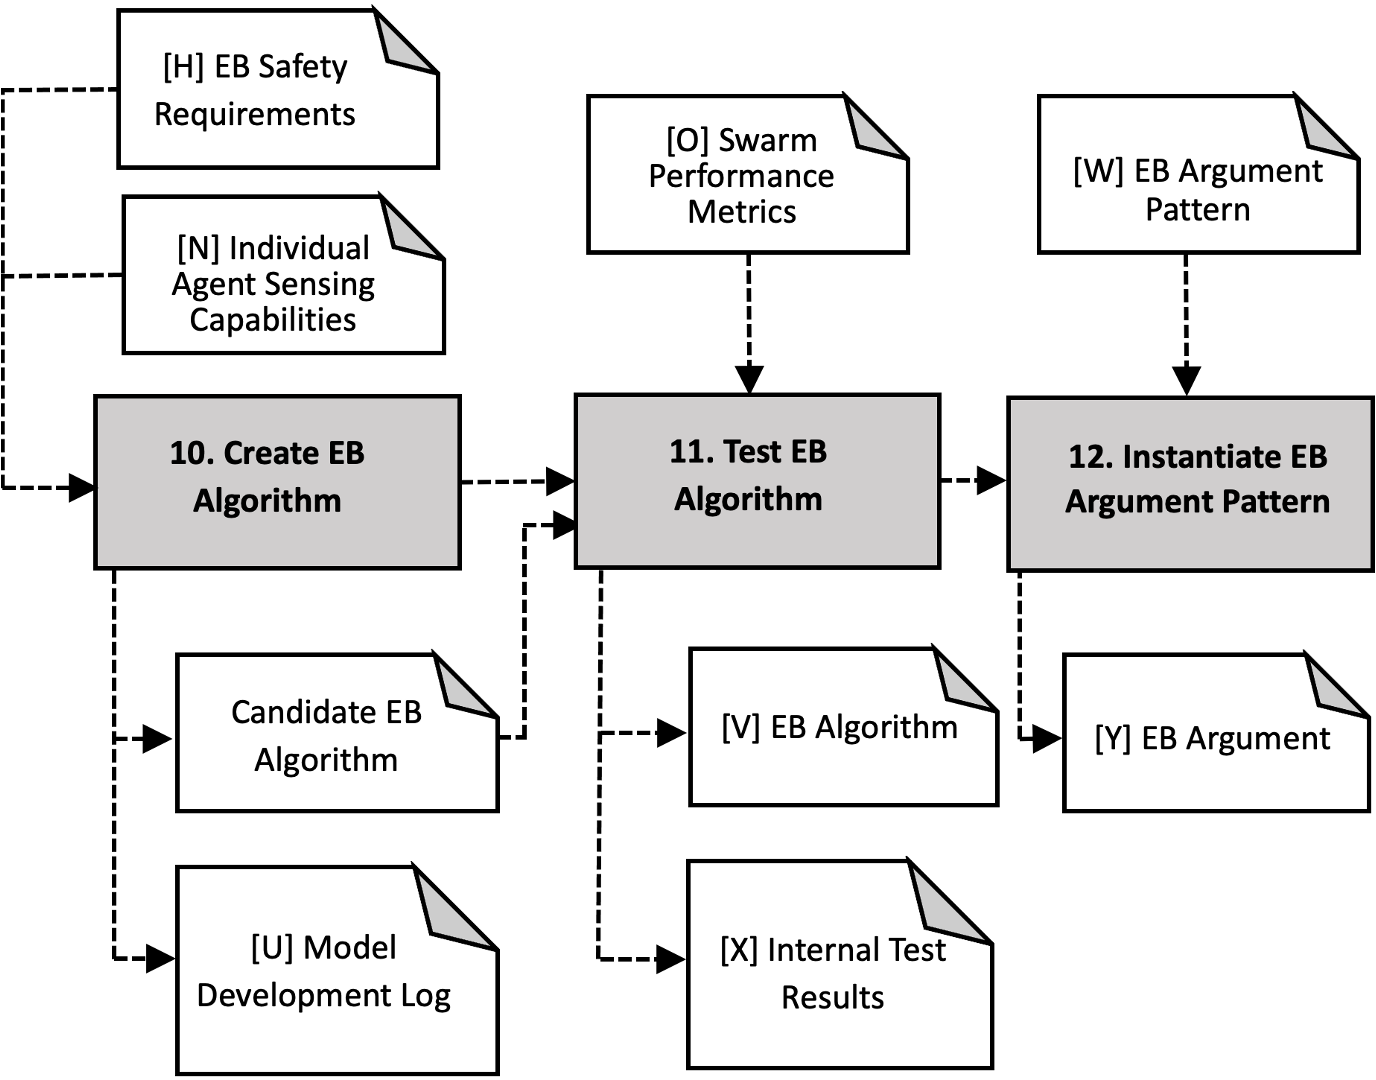
\includegraphics[width=0.5\textwidth]{figures/amlas-a-stage4-v2.png}%amlas-a-stage4.png
% 	\caption{Adapted AMLAS model learning process.}
% 	\label{amlas-a-stage4}
% \end{figure}

In the design of an emergent behaviour algorithm, the challenge is in selecting behaviours at the individual level of the agent which give rise to the desired emergent behaviour at the swarm level. The original AMLAS application in Stage 4 focused on the creation, testing and instantiation of a machine learning model for a single system with no emergent behaviours to consider for a collective. In our adaptation of AMLAS for the robot swarm,  we step away from the machine learning paradigm to allow consideration for all possible optimization algorithms which may attain the target emergent behaviour.

\begin{figure}[!h]
\centering
\begin{minipage}{.5\textwidth}
    \centering
    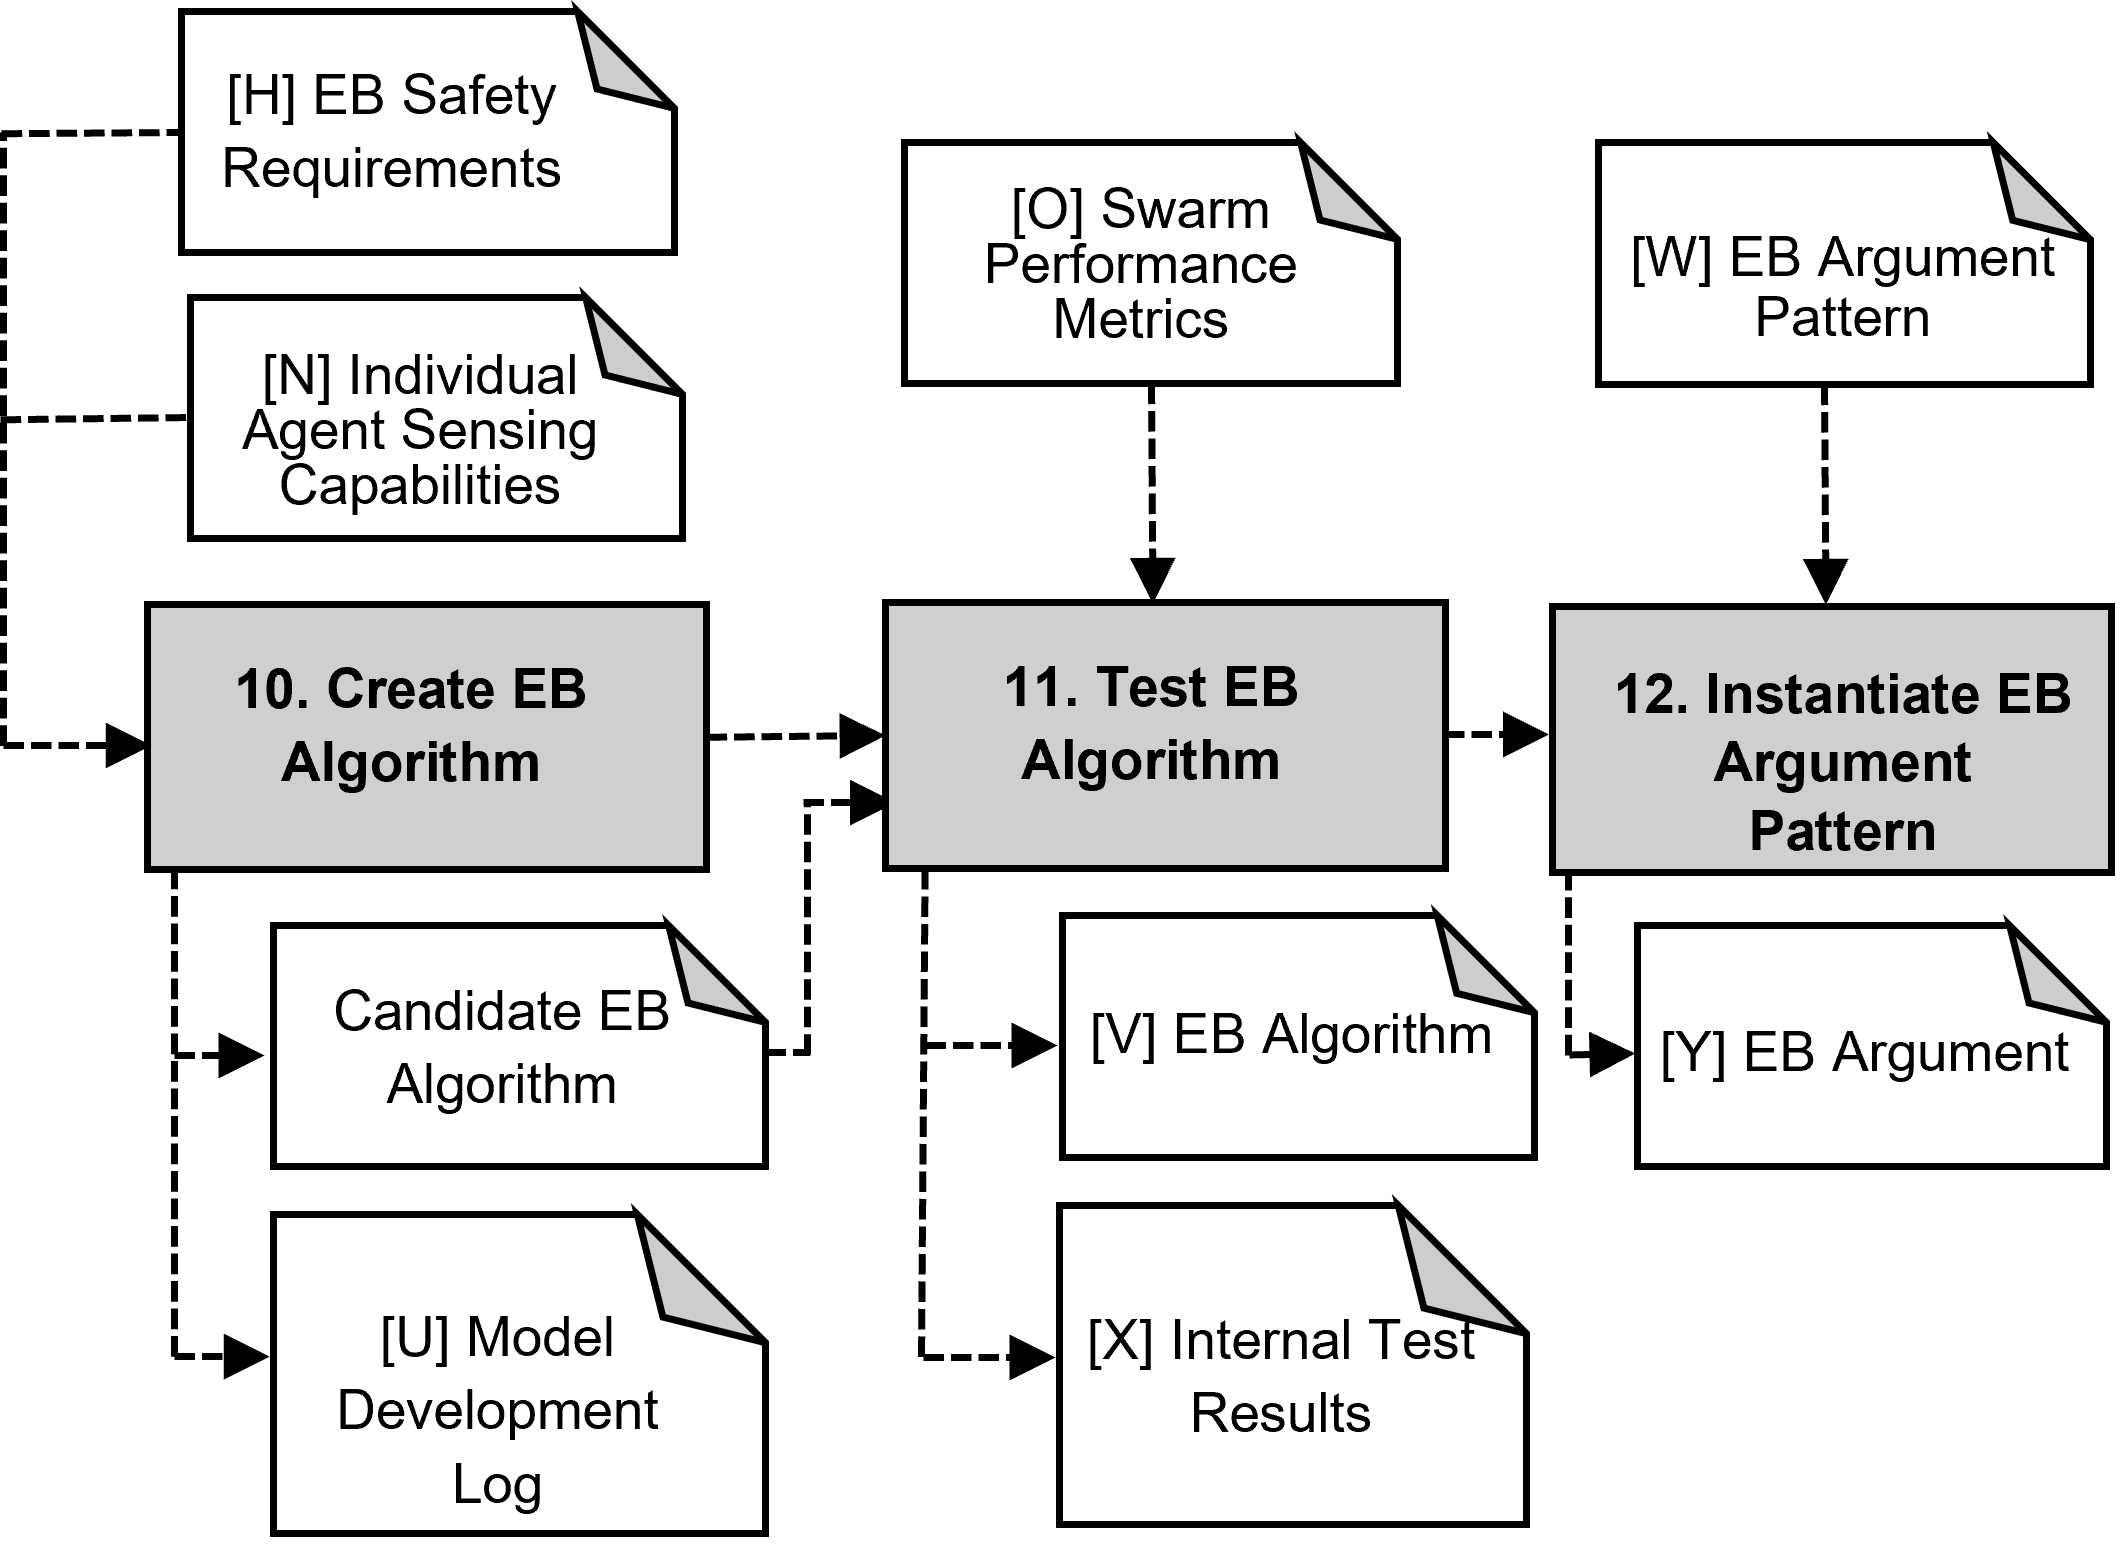
\includegraphics[scale=0.375]{figures/AMLAS-STAGE-4-V3.png}%amlas-a-stage4.png
    \caption{Adapted AMLAS model learning process.}
    \label{amlas-a-stage4}
\end{minipage}%
\begin{minipage}{.5\textwidth}
    \centering
    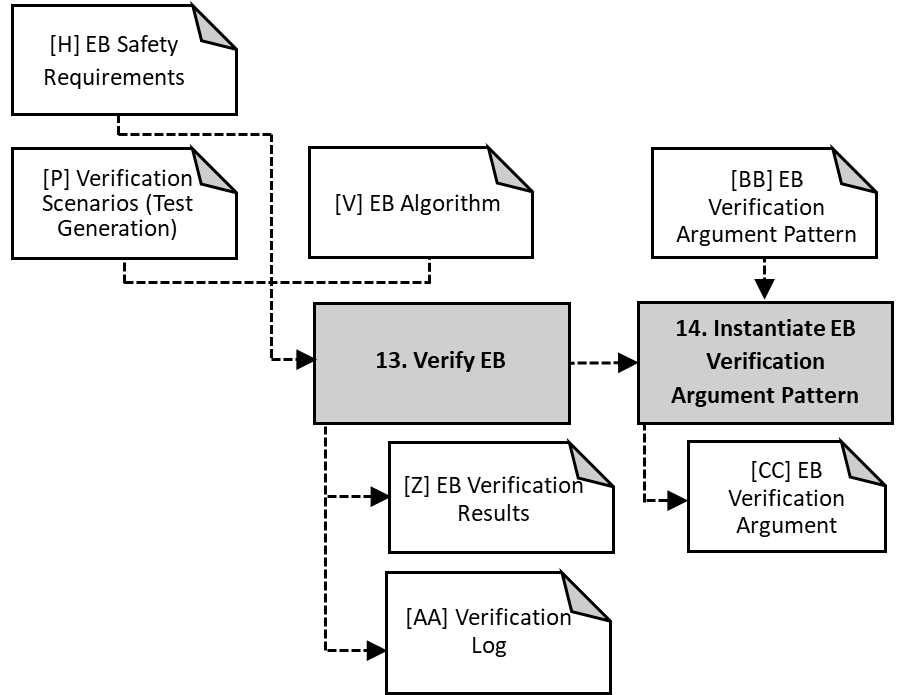
\includegraphics[scale=0.375]{figures/AMLAS-STAGE-5-V3.png}%amlas-a-stage5.png
    \caption{Adapted AMLAS verification assurance process.}
    \label{amlas-a-stage5}
\end{minipage}
\end{figure}

\subsubsection*{Activity 10. Create EB Algorithm}

Here we have two levels to consider: the individual level behaviour which is informed by agent sensing capabilities specified in [L.1], and the swarm level emergent behaviour which shall necessarily meet the safety requirements [H] defined in Stage 2 (see Fig.~\ref{amlas-a-stage4}). In the example of the cloakroom given in Section \ref{ex:cloakroom}, the target emergent behaviour for the swarm shall ensure that items are stored and retrieved by individuals. Performance requirements RQ1.1 and RQ1.2 specify an upper bound on the low/high impact collisions that a swarm shall experience in a given time frame. These requirements may be fulfilled by constraining the maximum velocity of individual robots, for example, or by ensuring that a robot has a camera or infra-red sensors enabling it to detect obstacles. The outputs from this activity follow the AMLAS framework, with a candidate emergent behaviour algorithm produced rather than a ML model. Output [U], the model development log, should log the rationale in the design process of the emergent behaviour algorithm.

\subsubsection*{Activity 11. Test EB Algorithm}

In this activity, the candidate emergent behaviour will be tested against the swarm performance metrics [O] produced in Stage 3. Testing ensures that the emergent behaviour performs as desired with respect to the defined metrics and in the case where performance is above the accepted thresholds, the emergent behaviour algorithm will be produced as an output [V] of the activity. The internal test results [X] will also be an output from the testing process.

\subsection{Stage 5: Model Verification} \label{framework-stage5}
%\noindent \textbf{\textit{[Lead:  WP4]}}\\ 
%\noindent\textbf{\textit{Author Guidelines: 900–1800 words / 1–2 pages (maximum); \\Format/structure: Describe adapted AMLAS activities, inputs and outputs using cloakroom case study examples. Activities: 13; Inputs: H, P, V; Outputs: Z, AA}}\\
%See Fig.~\ref{amlas-a-stage5} and Fig.~\ref{amlas-a-testbench}.	

% *****************
% GC Contribution, see table for qualities on `swarm' tab here:
% https://uob.sharepoint.com/:x:/r/teams/grp-TAS_Research2/Shared%20Documents/Verification/presentations/TrustQualities.xlsx?d=w4527b0bf0f4e49ab905d638dcb8c14ff&csf=1&web=1&e=8RW2vb

Inputs to the verification process are the [H] EB Safety Requirements, [P] Verification Scenarios (Test Generation) and [V] EB Algorithm (see Fig.~\ref{amlas-a-stage5}). 
%
The verification method and assessment process within that method will be largely determined by the specifics of the safety requirements. Some safety specifications lend themselves towards certain assessment methods due to the scenarios they prescribe.
%
For example, assessing the swarm system meets the requirements for performance given a motor fault injection [RQ1.6] may be easier to realise in physical or simulation based testing approaches, than constructing a reliable formal model of robot behaviour given the complex physical dynamics of a faulty wheel. 
%
However, when considering the adaptability requirements, a formal, probabilistic-based verification technique of the EB algorithm [V] is more suitable. For example, in [RQ2.1] analysis using a probabilistic finite state machine of the swarm behaviour (see \cite{Hoffmann2016,Calinescu2018}) could identify the dwell period within states. Monitors could be used to observe when agents enter a stationary state, e.g. \texttt{agent\_velocity=0 $\land $  t\_counter  $\ge$ 100}, and identify if time within that state exceeds some fixed value, and ascertain a probabilistic value to this metric.
%
%These examples will now be expanded in more detail below.
% \begin{figure}[!t]
% 	\centering
% 	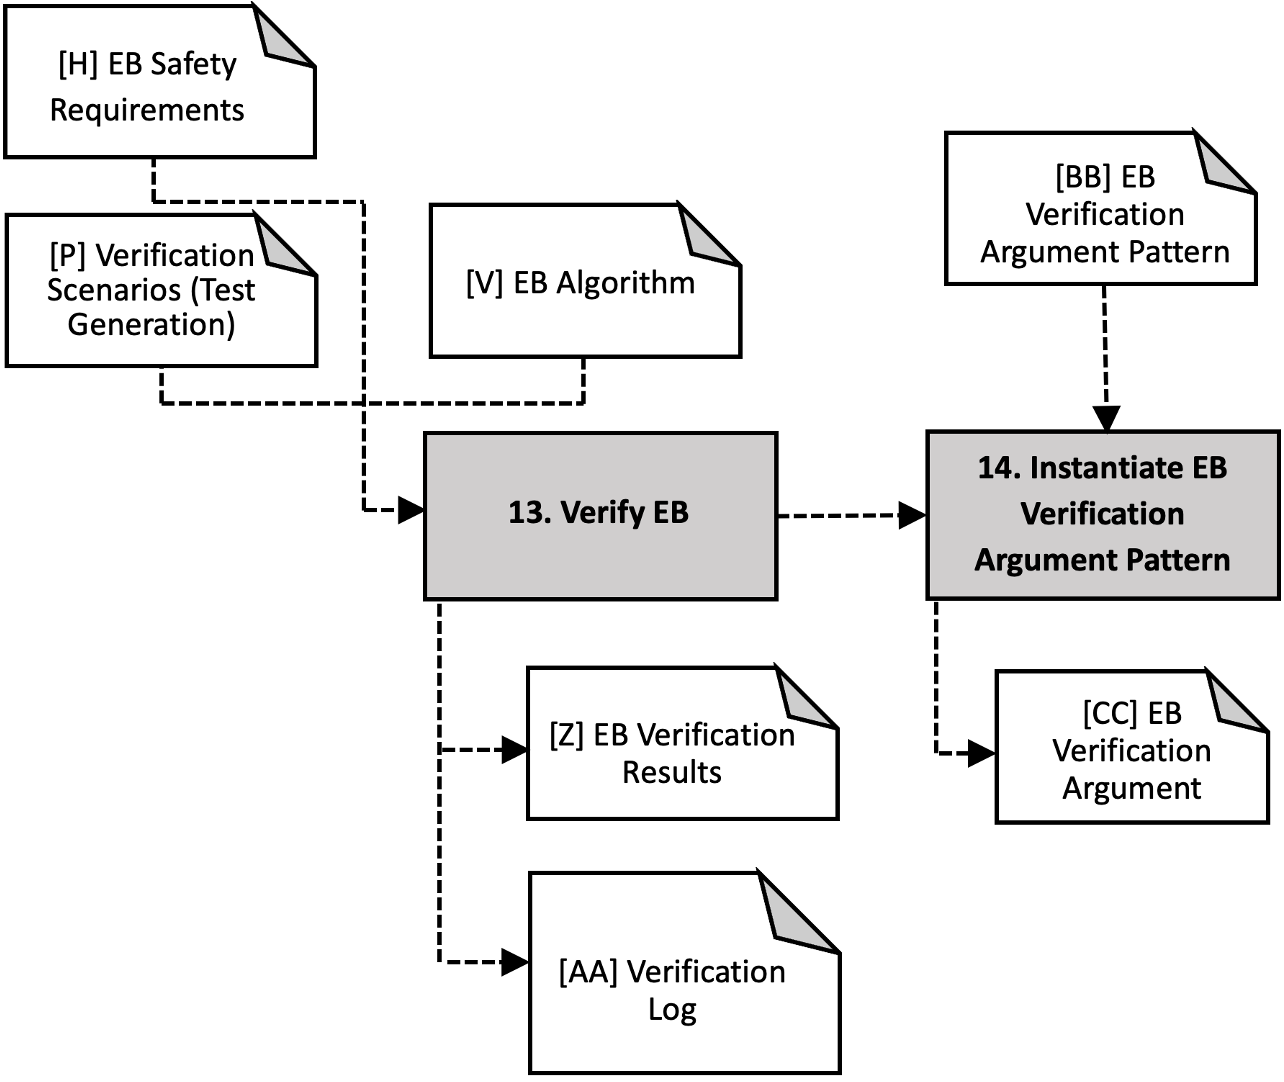
\includegraphics[width=0.5\textwidth]{figures/amlas-a-stage5_v2.png}%amlas-a-stage5.png
% 	\caption{Adapted AMLAS verification assurance process.}
% 	\label{amlas-a-stage5}
% \end{figure}
%\subsubsection*{[P] Verification Scenario (Test Generation)}

\textit{[P] Verification Scenario (Test Generation):} In most cases there will be multiple, valid verification scenarios, also called test cases, applicable for each of the safety specifications. A `good test case' must be \emph{effective} at finding bugs or defects, \emph{efficient} in minimising the number of tests required, use resources \emph{economically} and be \emph{robust} to system changes~\cite{Fewster1999}. 

%Using the EB Safety Requirements specification [H] and the principles of `good test cases', we have given an example here on how RQ2.2 might be appropriately verified.
% \paragraph*{RQ1.1 Low Impact collisions}

% For RQ1.1, relating to low impact collisions, suitable scenarios should consider a mix of both synthetic and physical testing to observe the safety compliance of the swarm controller. An important metric for assessing this safety requirement will be collision detection which could be achieved either through on-board hardware sensors or indirectly through external monitoring, e.g. overhead camera and tracking system. Simulation is a valid verification method for RQ1.1 as testing time can be accelerated through parallelisation and test generation could be automated to include some randomisation and constrained randomisation whilst monitoring the collision detection metric. Physical testing, usually limited due to time and cost constraints, should be more prescriptive and should orchestrate scenarios that have a high probability of exercising the collision detection routine of the swarm agent controller ([V] EB Algorithm), for example forcing swarm agents to travel a narrow passage to elevate swarm density. 

% Runtime verification can offer a solution to verifying systems that operate in large state-spaces, that may be intractable to verify at design time or through sampling the state space in testing. However, the choice or design of runtime oracle which provides the ground truth may require significant development, or innovative solutions~\cite{maple2020cyres}. For RQ1.1 runtime verification may be achieved with collision detection monitors, either internally with hardware or externally through a tracking system, e.g. Vicon. External systems may be less reliable that physical, on-board sensing, e.g. accelerometer based collision detection, but being an independent system offers other assurances such as being an independent evidence source and protection against cascading failure that fails to report the collision event, e.g. due to network connectivity failure.

% \paragraph*{RQ2.2 Agent Movement}

% This requirement ensures agents move every 100 seconds outside the delivery area, a suitable verification metric could monitor the time agents are outside a designated geospatial area (the delivery site) in addition to monitoring agent wheel speed. Scenarios should be biased towards these conditions by, for example, ensuring a sufficient number of agents outside the delivery area (by making the delivery area small or non-existent) and monitoring when wheel speed is zero for sufficiently long horizons to improve the likelihood of witnessing such an event by chance or by biasing events with adversarial agents, e.g. see~\cite{chance2020agency}. Increasing the chance that such rare events occur can accelerate evidence gathering which could be done in this case, for example, by constraining the agents environment, increasing swarm density, or fault injecting to the collision sensors so valid movement actions are limited.

% \begin{table*}[!t]
% 	\centering
% 	\begin{tabular}{llll}
% 		\textbf{RQ}   & \textbf{Verification Class}  & \textbf{Verification Method} & \textbf{Scenario} \\
% 		\hline
% 		1.1 	      & simulation 	   & constrained randomisation, directed tests & path intersection     \\
% 		low impact    & physical testing   & prescriptive trial 				       & path intersection	 \\
% 		collisions    & runtime		   & collision monitoring metric 		       & operational		 \\
% 		\hline
% 		2.2 	      & formal 	 	   & probabilistic finite state machine 	   & n/a      \\
% 		movement      & simulation 	   & constrained randomisation, directed tests & task representative     \\
% 		every 100s    & physical, runtime  & stationary monitoring metric 			   & operational		 \\
% 		\hline
% 	\end{tabular}
% 	\caption{Verification scenarios [P] and suitable methods.}\label{tab:testgen}
% \end{table*}

% \begin{figure*}[!t]
% 	\centering
% 	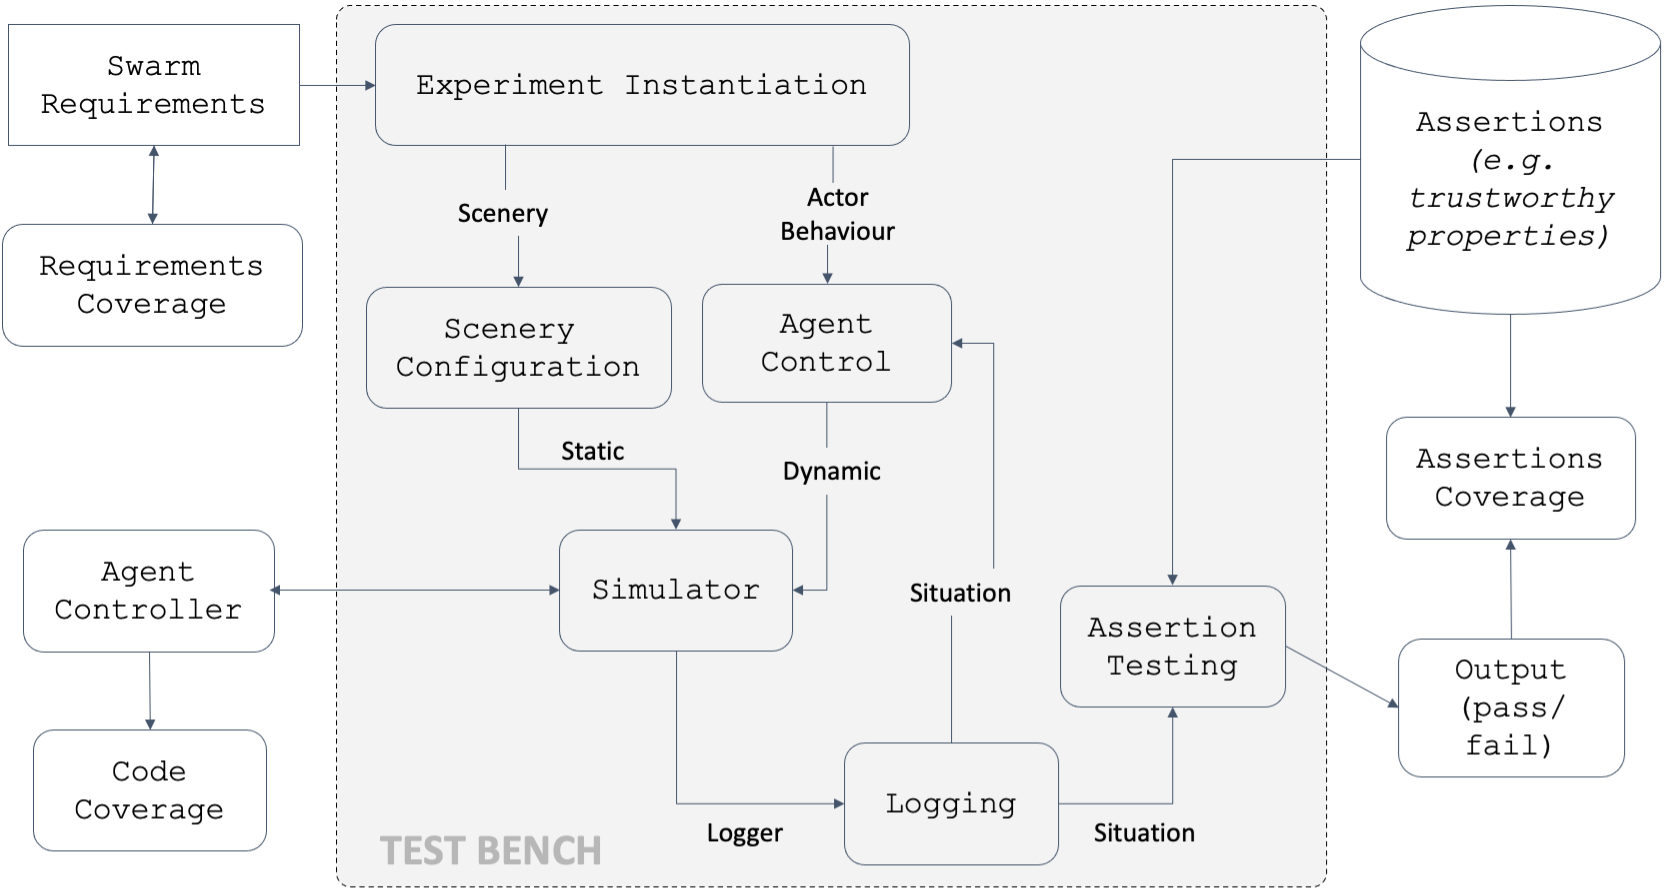
\includegraphics[width=1.0\textwidth]{figures/verification-testbench.png}
% 	\caption{Adapted AMLAS verification assurance process: test bench.}
% 	\label{amlas-a-testbench}
% \end{figure*}
% \\

% \subsubsection*{Verification Testbench}

% For simulation-based testing, a testbench can be used to orchestrate the `verify' task (activity 13 of AMLAS), see Fig.~\ref{amlas-a-testbench}. The testbench operates by using a \emph{simulator} to test the \emph{Agent Controller} software ([V] EB Algorithm) against \emph{Static} and \emph{Dynamic} stimuli. These stimuli are formed from \emph{Scenery} and \emph{Actor Behaviour} components which could be, for example, a virtual warehouse with staff, other robots and controllable lighting presenting a typical scenario to the virtual swarm. The \emph{Swarm Requirements} are used to drive suitable experiment instantiation so that the stimuli provoke the intended behaviours in the swarm that will prove (or possibly disprove) the safety properties under observation. A coverage monitor will be used to check that all the requirements have sufficient evidence against each entry and, for dynamic testbench architectures, can even be used to drive additional test cases. 

% In addition to requirements coverage, the there may also be coverage placed on the Agent Controller code itself, ensuring that all code is executed as expected for each behaviour. Assertions Coverage is a third method by which safety assurance evidence can be gathered. Assertions are statements pertaining to system properties written in the form of a ruleset, for example ``A swarm agent shall not collide with another swarm agent". Such an assertion can be monitored during verification activities, which is represented in the lower right section of the testbench. Through \emph{logging} the appropriate data channels, such as agent position and speed, and then analysing the data to perform \emph{Assertion Testing} either at runtime or offline, the swarm can be shown to comply with these assertions, e.g. see~\cite{harper2021safety}. \\



% \subsubsection*{Verifiability \& Visualisation}

% %Physical testing offers the opportunity to measure ground-truth..
% %Resolves the reality-gap to simulation...
% %Physical tends to take longer, cost more to acquire data...

% Verifiability is the process by which the verification task can be achieved with less effort through implementation of useful metrics and processes prior to the  development stage, i.e. at design time. Much effort goes into verifying systems that have already been developed, but by thinking how system properties can be observed or measured during the design stage and implementing these, will allow for greater transparency and explainability of the system to verification engineers and regulators. This could be creating software inspection points~\cite{koopman2018toward} giving visibility of decisions or actions taken by the system in a human-readable format. 

% Figure~\ref{swarm_trust_spider} is an example of a safety visualisation spider graph for a swarm, showing \emph{minimum} and \emph{acheived} levels of system properties, where minimum levels may be defined by standards or specifications. By considering verifiability, monitors could be included into the system to monitor events such as \emph{Task Performance}, \emph{Agent Uptime} and \emph{Collision Avoidance} rate. If the average \emph{Idle Rate} of the swarm was monitored then operators could identify optimal operational agent numbers for the swarm, and either add or remove agents as a direct response to this metric, to give optimal task performance. By visualising \emph{Network Connectivity} operators can be reassured of this function which builds trust in the safety of the system and helps debug the system if an error occurs. 

% \begin{figure}
% 	\centering
% 	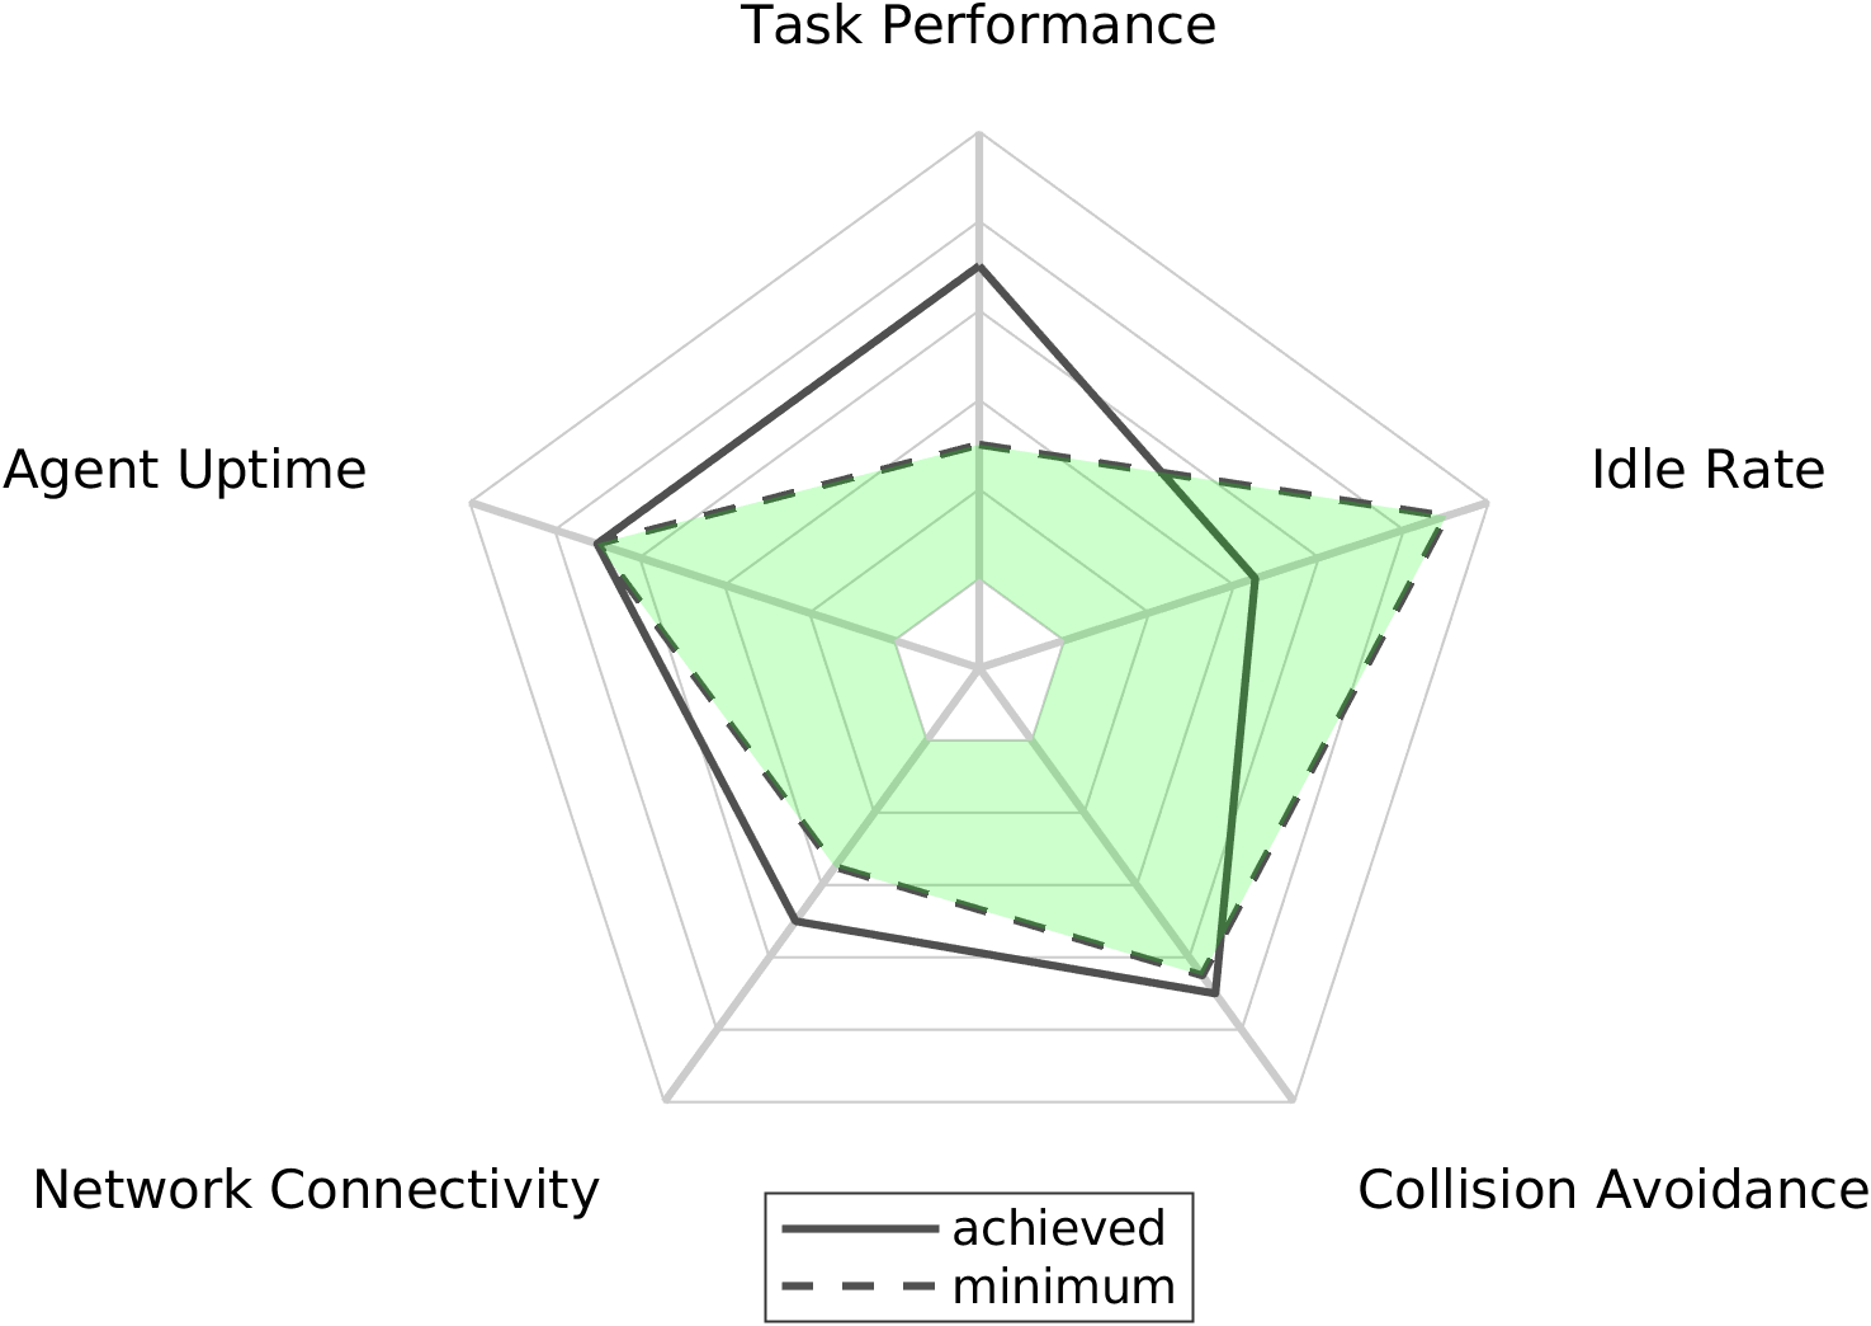
\includegraphics[width=0.5\textwidth]{figures/swarm_trust_spider.png}
% 	\caption{Visualising swarm safety properties.}
% 	\label{swarm_trust_spider}
% \end{figure}

%\begin{itemize}
%	\item Test bench for swarms
%	\item Probabilistic verification ideas
%	\item Simulation-based testing
%	\item Verifiability?
%\end{itemize}

\subsection{Stage 6: Model Deployment} \label{framework-stage6}
%\noindent \textbf{\textit{[Leads:  WP4 \& WP5; Additional: WP3]}}\\ 
%\noindent\textbf{\textit{Author Guidelines: 900–1800 words / 1–2 pages (maximum); \\Format/structure: Describe adapted AMLAS activities, inputs and outputs using cloakroom case study examples.\\ 
%\noindent WP5 = (Activities: 15, Inputs: V, A, B, C, D, Outputs: DD), \\
%\noindent WP4 = (Activities: 16, Inputs: EE, Outputs: FF), \\
%\noindent WP3 = (Regulatory Considerations – 675 words / 0.75 page maximum)}}\\
%See Fig.~\ref{amlas-a-stage6}

\subsubsection*{Activity 15. Integrate EB}

With the emergent behaviour verified, the next step is to take the model [V], safety requirements [A], environment description [B], and system description [C] and integrate the emergent behaviour with the system to be deployed (see Fig.~\ref{amlas-a-stage6}). 

In this activity we use the inputs to this stage to educate the implementation of the emergent behaviour and anticipate errors we might expect in the interactions between agents and the overall emergent behaviour. Despite the rigorous validation and testing conducted in previous stages, there will still be a gap between the test environment and the intended, every day use, deployed scenario. The output, [DD] Model Development Log, captures these anticipated gaps between testing and reality and the differences in behaviour that may surface. 
%For example, once physically deployed it may become apparent that large fluctuations in speed used to maintain performance while keeping the system safe for humans, may in reality be too much of a draw on the agents batteries to get a reasonable lifetime out of each battery charge. To address this, the behaviour may need to be tweaked to sacrifice some performance in the short term, reducing the rates of acceleration experienced by agents, in order to gain a longer battery life.

\begin{figure}[!t]
	\centering
	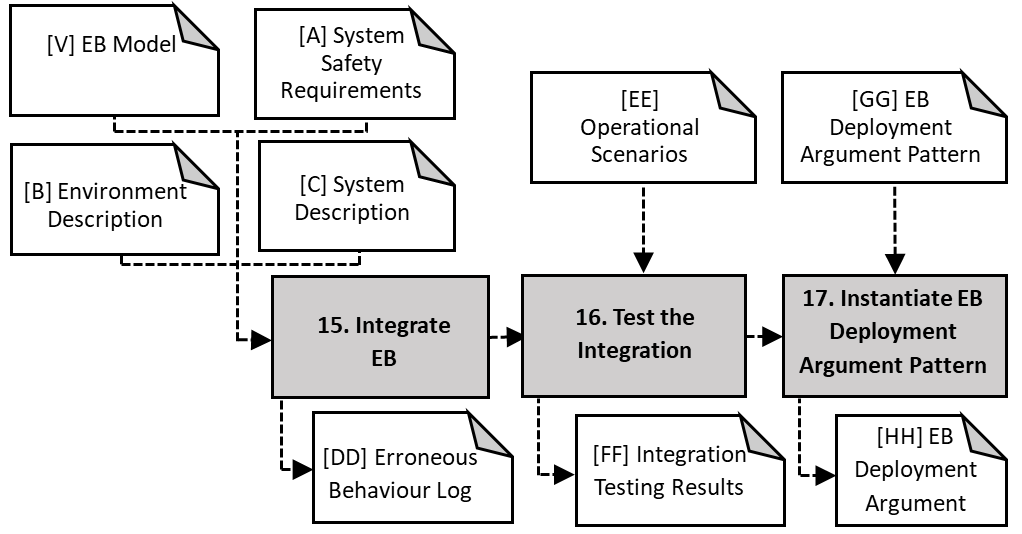
\includegraphics[width=0.6\textwidth]{figures/AMLAS-STAGE-6-V3.png}%amlas-a-stage6.png
	\caption{Adapted AMLAS model deployment assurance process.}
	\label{amlas-a-stage6}
\end{figure}
\subsubsection*{Activity 16. Test the Integration}

Once the initial integration is complete, the physical implementation should undergo additional testing in which the system will be observed in multiple operational scenarios, as specified in [EE].

%\paragraph*{[EE] Operational Scenarios}
\textit{[EE] Operational Scenarios:} These operational scenarios should reflect the environment descriptions specified in [B], offering a real-world situations to examine the behaviour of the integrated system. The testing of the integrated system in these true-to-operation environments should be conducted in a safe manner. Ensuring that the entire multi-agent system can be shut down in an emergency, or providing shadow operators for groups of agents, taking over should the swarm behave erroneously. In our use case, an example of [EE] may take the form of a small deployment of agents in a real but controlled storage area.

% Capture any integration issues

% provide a few environment examples

% Identify Erroneous behaviour expected and outlined in [DD], while simultaniously looking to catch/identify any issues of integration previously overlooked.

%\paragraph*{[FF] Integration Testing Results}
\textit{[FF] Integration Testing Results:} Results from the integration testing will be reported here, detailing how the system performs against the safety requirements [H] specified in stage 2.

%\subsection{Stage 7: Assurance Case}
	
\section{Discussion and Conclusions} \label{discussion-conclusions}

\section*{Acknowledgments}
The work presented in this paper has been supported by the UK Engineering and Physical Sciences Research Council (EPSRC) under the grant [EP/V026518/1].

%
% ---- Bibliography ----
%
% BibTeX users should specify bibliography style 'splncs04'.
% References will then be sorted and formatted in the correct style.
%

\bibliographystyle{splncs04}
\bibliography{AERoS-Bib}%{AssuranceFWK-Swarms-Bibliography}
%
\end{document}
